\section{KHÁI NIỆM VECTƠ}
\subsection{TÓM TẮT LÝ THUYẾT}
\subsubsection{Khái niệm vectơ}
Cho đoạn thẳng $AB$. Nếu chọn điểm $A$ làm điểm đầu, điểm $B$ làm điểm cuối thì đoạn thẳng $AB$ có hướng từ $A$  đến $B$. Khi đó ta nói $AB$ là một \indamm{đoạn thẳng có hướng}.	\\[0.2cm]
\iconMT~\indam{Định nghĩa}
\begin{boxdn}
	\begin{itemize}
		\item  \indamm{Vectơ} là một đoạn thẳng có hướng, nghĩa là trong hai điểm mút của đoạn thẳng đã chỉ rõ điểm đầu, điểm cuối.
		\item  Độ dài của vectơ là khoảng cách giữa điểm đầu và điểm cuối của vectơ đó.
	\end{itemize}
\end{boxdn}

\begin{note}
	\immini{
		\begin{itemize}
			\item Nếu chỉ rõ điểm đầu là $A$ và điểm cuối là $B$, ta có \lq\lq vectơ $AB$\rq\rq, kí hiệu $\overrightarrow{AB}$. 
			\item Nếu không cần chỉ rõ điểm đầu và điểm cuối, ta dùng các chữ cái thường để kí hiệu. Ví dụ $\overrightarrow{a}$, $\overrightarrow{b}$, $\overrightarrow{x},\ldots$
			\item  Đường thẳng đi qua hai điểm $A$ và $B$ gọi là \indamm{giá} của $\overrightarrow{AB}$.
			\item Độ dài của đoạn thẳng $AB$ gọi là \indamm{độ dài} của $\overrightarrow{AB}$, kí hiệu là $\left|\overrightarrow{AB}\right|=AB$. 
	\end{itemize}	}{
		\begin{tikzpicture}[smooth,samples=300,scale=0.8,>=stealth]
			\path 
			(0,0) coordinate (A)
			(3,1.3) coordinate (B)
			(1,-0.5) coordinate (X)
			(3.5,-0.5) coordinate (Y)
			;
			\draw[thick,-{Stealth[length=2.5mm]}] (X)--(Y);
			\draw[thick,-{Stealth[length=2.5mm]}] (A)--(B);
			\draw ($(X)!0.5!(Y)$) node[shift=(90:0.25)] {$\overrightarrow{x}$};
			\foreach \x/\g in {A/-90,B/90}
			\draw[fill=black] (\x) circle (.036)+(\g:.35)
			node{$\x$};	
	\end{tikzpicture}}
\end{note}


\subsubsection{Hai vectơ cùng phương, cùng hướng}
\iconMT~\indam{Định nghĩa}
\begin{boxdn}
	\begin{itemize}
		\item Hai vectơ được gọi là \indamm{cùng phương} nếu giá của chúng \textit{song song} hoặc \textit{trùng nhau}.
		\item Nếu hai vectơ cùng phương thì chúng có thể \indamm{cùng hướng} hoặc \indamm{ngược hướng}.
	\end{itemize}
\end{boxdn}

\begin{note}
	\indamm{Điều kiện để ba điểm thẳng hàng}\\[0.2cm]
	Ba điểm phân biệt $A$, $B$, $C$ thẳng hàng khi và chỉ khi $\overrightarrow{AB}$ và $\overrightarrow{AC}$ cùng phương.
\end{note}

\subsubsection{Hai vectơ bằng nhau}
\iconMT~\indam{Định nghĩa}
\begin{boxdn}
	Hai vectơ $\overrightarrow{a}$ và $\overrightarrow{b}$ được gọi là \indamm{bằng nhau}, kí hiệu $\overrightarrow{a}=\overrightarrow{b}$ nếu chúng \indamm{có cùng hướng} và \indamm{cùng độ dài.}
\end{boxdn}

\subsubsection{Hai vectơ đối nhau}
\iconMT~\indam{Định nghĩa}
\begin{boxdn}
	Hai vectơ $\overrightarrow{a}$ và $\overrightarrow{b}$ được gọi là \indamm{đối nhau}, kí hiệu $\overrightarrow{a}=-\overrightarrow{b}$ nếu chúng \indamm{ngược hướng} và có \indamm{cùng độ dài.}
\end{boxdn}

\subsubsection{Vectơ-không}
\iconMT~\indam{Định nghĩa}
\begin{boxdn}
	Vectơ-không là vectơ có điểm đầu và điểm cuối trùng nhau, kí hiệu là $\overrightarrow{0}$ (hoặc $\overrightarrow{AA}$).
\end{boxdn}

\begin{note}
	\begin{itemize}
		\item Quy ước vectơ-không có độ dài bằng $0$.
		\item Vectơ-không luôn cùng phương, cùng hướng với mọi vectơ.
		\item Mọi vectơ-không đều bằng nhau, ta có $\overrightarrow{0}=\overrightarrow{AA}=\overrightarrow{BB}=\overrightarrow{CC}=\ldots$ với mọi điểm $A$, $B$, $C$, $\ldots$
		\item Vectơ đối của vectơ-không là chính nó.
	\end{itemize}
\end{note}

\subsection{RÈN LUYỆN KĨ NĂNG GIẢI TOÁN}

\begin{dang}{Xác định vectơ; xác định phương và hướng của vectơ}
\end{dang}
%%=====VD1=======%%
\begin{vd}%[Dự án đề cương 3 Khối NH24-25-Dot1-Nguyễn Tấn Tài]%[0H5N1-1]
	\immini{Cho tam giác $ABC$. Hãy kể tên các vectơ (khác $\overrightarrow{0}$) có điểm đầu và điểm cuối là các đỉnh của tam giác.}{
		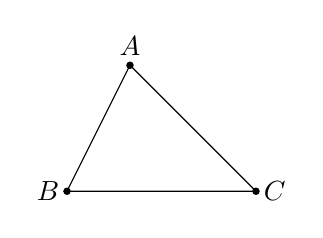
\begin{tikzpicture}[smooth,scale=0.8]
			\path
			(0,0) coordinate (B)
			(3,0) coordinate (C)
			(1,2) coordinate (A);
			\draw (A)--(B)--(C)--(A);
			\foreach \x/\g in {A/90,B/180,C/0} \draw [fill=black] (\x) circle (.05) + (\g:.3) node{$\x$};
	\end{tikzpicture}}
	\loigiai{
		Các vectơ có thể là $\overrightarrow{AB}$, $\overrightarrow{BA}$, $\overrightarrow{AC}$, $\overrightarrow{CA}$, $\overrightarrow{BC}$, $\overrightarrow{CB}$.}
\end{vd} 
\dongcham{3}
%%=====VD2=======%%
\begin{vd}%[Dự án đề cương 3 Khối NH24-25-Dot1-Nguyễn Tấn Tài]%[0H5H1-2]
	\immini{Cho hình bình hành $ABCD$ tâm $O$ như hình bên. 
		\begin{enumerate}
			\item Kể tên 2 vectơ cùng phương với vectơ $\overrightarrow{OA}$.
			\item Kể tên vectơ cùng hướng, ngược hướng với vectơ $\overrightarrow{OB}$.
		\end{enumerate}
	}{
		\begin{tikzpicture}[smooth,font=\footnotesize,scale=0.6]
			\path
			(0,0) coordinate (A)
			(1,2) coordinate (B)
			(4,2) coordinate (C)
			(3,0) coordinate (D);
			\coordinate (O) at ($(C)!0.5!(A)$);
			\draw (A)--(B)--(C)--(D)--cycle (A)--(C) (B)--(D);
			\foreach \x/\g in {A/-90,B/90,C/90,D/-90,O/90} \draw [fill=black] (\x) circle (.05) + (\g:.3) node{$\x$};
	\end{tikzpicture}}
	\loigiai{
		\begin{enumerate}
			\item Hai vectơ cùng phương với $\overrightarrow{OA}$ là $\overrightarrow{AC}$, $\overrightarrow{OC}$.\\
			Ngoài ra còn có $\overrightarrow{CA}$, $\overrightarrow{AO}$, $\overrightarrow{CO}$...
			\item Vectơ cùng hướng với $\overrightarrow{OB}$ là $\overrightarrow{DB}$, $\overrightarrow{DO}$;\\
			Vectơ ngược hướng với $\overrightarrow{OB}$ là $\overrightarrow{BO}$, $\overrightarrow{OD}$ và $\overrightarrow{BD}$.
	\end{enumerate}}
\end{vd} \dongcham{6}
%%=====Dạng 2=======%%
\begin{dang}{Hai vectơ bằng nhau, đối nhau}
\end{dang}
%%=====VD3=======%%
\begin{vd}%[Dự án đề cương 3 Khối NH24-25-Dot1-Nguyễn Tấn Tài]%[0H5N1-3]
	\immini{Cho tam giác $ABC$. Các điểm $M$, $N$ và $K$ lần lượt là trung điểm của $AB$, $AC$ và $BC$.
		\begin{enumerate}
			\item Tìm các vectơ bằng với $\overrightarrow{AM}$.
			\item Tìm các vectơ bằng với $\overrightarrow{KN}$.
	\end{enumerate}}{\hspace{1cm}
		\begin{tikzpicture}[scale=0.8, line join=round, line cap=round]
			\tkzDefPoints{0/0/A,1/2/B,4/0/C}
			\coordinate (M) at ($(A)!0.5!(B)$);
			\coordinate (N) at ($(C)!0.5!(A)$);
			\coordinate (K) at ($(B)!0.5!(C)$);
			\tkzDrawSegments(A,B B,C C,A M,N N,K M,K)
			\tkzDrawPoints[size=2,fill=black](A,B,C,M,N,K)
			\tkzLabelPoints[below, font=\footnotesize](A,N,C)
			\tkzLabelPoints[above, font=\footnotesize](B)
			\tkzLabelPoints[above left, font=\footnotesize](M)
			\tkzLabelPoints[above right, font=\footnotesize](K)
	\end{tikzpicture}}
	\loigiai{
		\begin{enumerate}
			\item Vì $M$ là trung điểm của $AB$ nên vectơ bằng với $\overrightarrow{AM}$ là $\overrightarrow{MB}$.\\
			Vì $NK$ là đường trung bình của $\triangle ABC$ nên vectơ bằng với $\overrightarrow{AM}$ là $\overrightarrow{NK}$.
			\item Vì $NK$ là đường trung bình của $\triangle ABC$ nên vectơ bằng với $\overrightarrow{KN}$ là $\overrightarrow{BM}$ và $\overrightarrow{MA}$.
		\end{enumerate}
	}
\end{vd} \dongcham{6}
%%=====VD4=======%%
\begin{vd}%[Dự án đề cương 3 Khối NH24-25-Dot1-Nguyễn Tấn Tài]%[0H5H1-3]
	\immini{Cho lục giác đều $ABCDEF$ tâm $O$.
		\begin{enumerate}
			\item Tìm các vectơ bằng với $\overrightarrow{EF}$.
			\item Tìm các vectơ là vectơ đối của $\overrightarrow{OB}$.
	\end{enumerate}}{\hspace{1cm}
		\begin{tikzpicture}[scale=0.7]
			\tkzDefPoint(0,0){O}
			\tkzDefPoint(2,0){E}
			\tkzDefPointBy[rotation=center O angle 60](E) \tkzGetPoint{F}
			\tkzDefPointBy[rotation=center O angle 120](E) \tkzGetPoint{A}
			\tkzDefPointBy[rotation=center O angle 180](E) \tkzGetPoint{B}
			\tkzDefPointBy[rotation=center O angle 240](E) \tkzGetPoint{C}
			\tkzDefPointBy[rotation=center O angle 300](E) \tkzGetPoint{D}
			\tkzDrawPoints[size=2,fill=black](A,B,C,D,E,F,O)
			\tkzDrawSegments(A,B B,C C,D D,E E,F F,A A,D F,C B,E)
			\draw (A) node[above] {$A$} (B) node[left] {$B$} (C) node[below] {$C$} (D) node[below] {$D$} (E) node[right] {$E$} (F) node[above] {$F$} (O) node[below left] {$O$};
		\end{tikzpicture}
	}
	\loigiai{
		\begin{enumerate}
			\item Các vectơ bằng với $\overrightarrow{EF}$ là $\overrightarrow{CB}$, $\overrightarrow{OA}$, $\overrightarrow{DO}$.
			\item Các vectơ đối của $\overrightarrow{OB}$ là $\overrightarrow{AF}$, $\overrightarrow{OE}$, $\overrightarrow{CD}$.
		\end{enumerate}
	}
\end{vd} \dongcham{6}

%%=====Dạng 3=======%%
\begin{dang}{Độ dài vectơ}
	Độ dài của $\overrightarrow{AB}$ là độ dài đoạn thẳng $AB$. Khi tính toán, ta có thể chú ý đến định lý Pythagore và các tỉ số lượng giác của góc nhọn trong tam giác vuông.
\end{dang}
%%=====VD5=======%%
\begin{vd}%[Dự án đề cương 3 Khối NH24-25-Dot1-Nguyễn Tấn Tài]%[0H5H1-5]
	\immini{Cho hình vuông $ABCD$ tâm $O$, cạnh bằng $2$. 
		\begin{enumerate}
			\item Tính độ dài của các vectơ $\overrightarrow{AB}$, $\overrightarrow{AC}$ và $\overrightarrow{AO}$.
			\item Gọi $I$ là trung điểm của $BC$. Tính độ dài của $\overrightarrow{AI}$.
		\end{enumerate}
	}{\hspace{1cm}
		\begin{tikzpicture}[smooth,font=\footnotesize,scale=1]
			\path
			(0,0) coordinate (A)
			(2,0) coordinate (B)
			(2,2) coordinate (C)
			(0,2) coordinate (D);
			\coordinate (O) at ($(B)!0.5!(D)$);
			\draw (A)--(B)--(C)--(D)--(A) (A)--(C) (B)--(D);
			\foreach \x/\g in {A/-90,B/-90,C/90,D/90,O/0} \draw [fill=black] (\x) circle (.045) + (\g:.3) node{$\x$};
		\end{tikzpicture}
	}
	\loigiai{
		\begin{center}
			\begin{tikzpicture}[smooth,font=\footnotesize,scale=1]
				\path
				(0,0) coordinate (A)
				(2,0) coordinate (B)
				(2,2) coordinate (C)
				(0,2) coordinate (D);
				\coordinate (I) at ($(B)!0.5!(C)$);
				\coordinate (O) at ($(B)!0.5!(D)$);
				\draw (A)--(B)--(C)--(D)--(A) (A)--(C) (B)--(D) (A)--(I);
				\foreach \x/\g in {A/-90,B/-90,C/90,D/90,O/0,I/0} \draw [fill=black] (\x) circle (.045) + (\g:.3) node{$\x$};
			\end{tikzpicture}
		\end{center}
		\begin{enumerate}
			\item Độ dài của $\overrightarrow{AB}$ là $\left|\overrightarrow{AB}\right|=AB=2$.\\
			Độ dài của $\overrightarrow{AC}$ là $\left|\overrightarrow{AC}\right|=AC=AB\cdot\sqrt{2}=2\sqrt{2}$.\\
			Độ dài của $\overrightarrow{AO}$ là $\left|\overrightarrow{AO}\right|=AO=\dfrac{AB\cdot\sqrt{2}}{2}=\sqrt{2}$.
			\item 
			Vì $I$ là trung điểm của $BC$ nên $IB=\dfrac{BC}{2}=1$.\\
			Vì $\triangle ABI$ vuông tại $B$ nên $AI=\sqrt{AB^2+BI^2}=\sqrt{2^2+1^2}=\sqrt{5}$.\\
			Độ dài của $\overrightarrow{AI}$ là $\left|\overrightarrow{AI}\right|=AI=\sqrt{5}$.
		\end{enumerate}
	}
\end{vd} \dongcham{5}
%%=====VD6=======%%
\begin{vd}%[0H5V1-5]
	Cho tam giác $ABC$ đều, cạnh bằng $3$. Gọi $H$ là trung điểm của $BC$ và $G$ là trọng tâm tam giác $ABC$.
	\begin{enumerate}
		\item Hãy tính độ dài của  $\overrightarrow{AH}$.
		\item Hãy tính độ dài của  $\overrightarrow{GB}$.
	\end{enumerate}
	\loigiai{
		\begin{center}
			\begin{tikzpicture}[scale=1.2,font=\footnotesize]
				\path (0,0) coordinate (B)--++(0:3) coordinate (C) --++(120:3) coordinate (A);
				\coordinate (H) at ($(B)!0.5!(C)$);
				\coordinate (G) at ($(A)!2/3!(H)$);
				
				% Vẽ tam giác và các đoạn thẳng cần thiết
				\draw (A)--(B)--(C)--cycle;
				\draw (A)--(H);
				\draw (A)--(G);
				
				% Vẽ điểm
				\foreach \point/\pos in {A/above,B/below,C/below,H/below right,G/right}
				\filldraw (\point) circle (1pt) node[\pos]{$\point$};
			\end{tikzpicture}
		\end{center}
		\begin{enumerate}
			\item Vì $\triangle ABC$ đều có cạnh $3$ nên $AB=BC=3$. Suy ra $BH=\dfrac{BC}{2}=\dfrac{3}{2}$.\\
			Mặt khác $AH$ cũng là đường cao của $\triangle ABC$ nên $AH \perp BC$.\\ 
			Xét $\triangle AHB$ vuông tại $H$ có $AH=\sqrt{AB^2-HB^2}=\sqrt{3^2-\left(\dfrac{3}{2}\right)^2}=\dfrac{3\sqrt{3}}{2}$.\\
			Vậy $\left|\overrightarrow{AH}\right|=\dfrac{3\sqrt{3}}{2}$.
			\item Vì $G$ là trọng tâm của $\triangle ABC$ nên $GH=\dfrac{1}{3}AH=\dfrac{\sqrt{3}}{2}$.\\
			Xét $\triangle GHB$ vuông tại $H$ có $GB=\sqrt{GH^2+HB^2}=\sqrt{\left(\dfrac{\sqrt{3}}{2}\right)^2+\left(\dfrac{3}{2}\right)^2}=\sqrt{3}$.\\ 
			Vậy $\left|\overrightarrow{GB}\right|=GB=\sqrt{3}$.
		\end{enumerate}
	}
\end{vd} \dongcham{13}
\subsection{BÀI TẬP TRẮC NGHIỆM}
\ind{PHẦN I.} \inden{Câu trắc nghiệm nhiều phương án lựa chọn. Mỗi câu hỏi học sinh chỉ chọn một phương án.}\\
\setcounter{ex}{0}
\Opensolutionfile{ans}[ans/0H5-B1-1]
\setcounter{ex}{0}
%%=======Câu 1=======%%
\begin{ex}%[0H5N1-1]%[Dự án đề kiểm tra Toán 10 GHKII NH24-25-lamnguyen]%[THPT Nguyen Thái Bình]
	\textit{(Trích đề HKI - THPT Nguyễn Thái Bình - Năm học 2024 - 2025)}
	\\	Vectơ có điểm đầu $D$, điểm cuối $E$ được kí hiệu là
	\choice
	{$\overrightarrow{ED}$}
	{\True $\overrightarrow{DE}$}
	{$\overline{DE}$}
	{$\left| \overrightarrow{DE}\right| $}
	\loigiai{
		Vectơ có điểm đầu $D$, điểm cuối $E$ được kí hiệu là $\overrightarrow{DE}$.
	}
\end{ex}
%%=======Câu 2=======%%
\begin{ex}%[0H5N1-2]%[Dự án đề kiểm tra Toán 10 HKI NH24-25 - Quan Ón]%[THPT HỒ THỊ BI - Tp.HCM]
	\textit{(Trích đề HKI - THPT Hồ Thị Bi - Năm học 2024 - 2025)}\\	Cho hình bình hành $ABCD$. Có bao nhiêu vectơ khác vectơ-không cùng phương với $\overrightarrow{AB}$ có điểm đầu và cuối là các đỉnh của hình bình hành?
	\choice
	{\True $3$}
	{$4$}
	{$6$}
	{$5$}
	\loigiai{
		Các vectơ khác vectơ-không cùng phương vectơ $\overrightarrow{AB}$ là  $\overrightarrow{BA}$, $\overrightarrow{CD}$ và $\overrightarrow{DC}$.
	}
\end{ex}
%%=======Câu 3=======%%
\begin{ex} %[0H5N1-2] %[0D6H3-5]%[Dự án đề kiểm tra Toán 10 HKI NH24-25- Nguyễn Tấn Tài]%[THPT TX Quảng Trị]
	\textit{(Trích đề HKI - THPT TX Quảng Trị - Năm học 2024 - 2025)}\\	Cho ba điểm $M, N, P$ thẳng hàng, trong đó $N$ nằm giữa hai điểm $M$ và $P$. Khi đó cặp vectơ nào sau đây cùng hướng?
	\choice
	{$\vec{MP}$ và $\vec{PN}$}
	{$\vec{MN}$ và $\vec{PN}$}
	{$\vec{NP}$ và $\vec{NM}$}
	{\True $\vec{MN}$ và $\vec{MP}$}
	\loigiai{
		\begin{center}
			\begin{tikzpicture}[line join=round, line cap=round,>=stealth,font=\footnotesize,scale=1]
				\draw (0,0) coordinate (M) --++(0:2) coordinate (N)--++(0:3) coordinate(P);
				\foreach\x/\g in {M/90, N/90, P/90}{
					\draw[fill=black] (\x) circle (1pt)+(\g:0.3) node {$\x$};
				};
			\end{tikzpicture}
		\end{center}
		$\vec{MN}$ và $\vec{MP}$ cùng hướng.
	}
\end{ex}
%%=======Câu 4=======%%
\begin{ex}%[0H5N1-3]%[Dự án đề kiểm tra Toán 10 HKI NH24-25 - Quan Ón]%[THPT HỒ THỊ BI - Tp.HCM]
	\textit{(Trích đề HKI - THPT Hồ Thị Bi - Năm học 2024 - 2025)}	\immini{
		Cho lục giác đều $ABCDEF$ tâm $O$. Hãy tìm các vectơ khác vectơ-không có điểm đầu, điểm cuối là đỉnh của lục giác và tâm $O$ sao cho bằng với $\overrightarrow{AB}$.
		\choice
		{\True $\overrightarrow{FO}$, $\overrightarrow{OC}$, $\overrightarrow{ED}$}
		{$\overrightarrow{BO}$, $\overrightarrow{OC}$, $\overrightarrow{ED}$}
		{$\overrightarrow{FO}$, $\overrightarrow{AC}$, $\overrightarrow{ED}$}
		{$\overrightarrow{FO}$, $\overrightarrow{OC}$, $\overrightarrow{FD}$}
	}
	{
		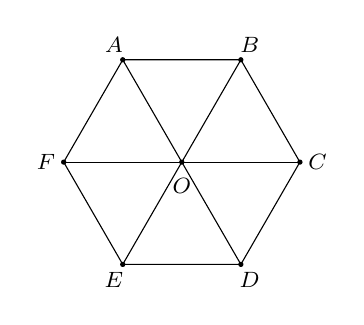
\begin{tikzpicture}[scale=0.75, font=\footnotesize, line join=round, line cap=round, >=stealth]
			\def\r{2}
			\path (0,0) coordinate (O);
			\foreach\x/\y in {A/120,B/60,C/0,D/-60,E/-120,F/180}
			{\path (\y:\r) coordinate (\x);
				\draw (O)--(\x);
				\draw[fill=black] (\x) circle (1pt)+(\y:0.3) node{$\x$};
			}
			\draw (A)--(B)--(C)--(D)--(E)--(F)--(A);
			\draw[fill=black] (O) circle (1pt)+(-90:0.4) node{$O$};
		\end{tikzpicture}
	}
	\loigiai{
		Các vectơ khác vectơ-không bằng với $\overrightarrow{AB}$ là các vectơ $\overrightarrow{FO}$, $\overrightarrow{OC}$, $\overrightarrow{ED}$.
	}
\end{ex}
%%=======Câu 5=======%%
\begin{ex}%[0H5N1-5]%[Dự án đề kiểm tra Toán 10 HKI NH24-25- Nguyễn Trần Phong]%[THPT Chuyên Trần Phú - Hải Phòng]
	\textit{(Trích đề HKI - THPT Chuyên Trần Phú, Hải Phòng - Năm học 2024 - 2025)}\\	Mệnh đề nào sau đây \textbf{sai}?
	\choice
	{$|\overrightarrow{A B}|=|\overrightarrow{B A}|$}
	{Vectơ $\overrightarrow{0}$ cùng hướng với mọi vectơ}
	{\True $\overrightarrow{A A}=0$}
	{Vectơ $\overrightarrow{0}$ cùng phương với mọi vectơ}
	\loigiai{
		Ta có $\overrightarrow{A A}=\overrightarrow{0}$ nên mệnh đề $\overrightarrow{A A}=0$ sai.
	}
\end{ex}
%%=======Câu 6=======%%
\begin{ex}%[0H5H1-5]%[Dự án đề kiểm tra Toán khối 10 học kì 1 NH24-25-Dot 4-Thái Bảo ]%[THPT Nguyễn Thị Minh Khai  - TpHCM]
	\textit{(Trích đề HKI - THPT Nguyễn Thị Minh Khai - Năm học 2024 - 2025)}\\	Cho hình chữ nhật $ABCD$ có $AB=a$, $AD=2a$. Tính $\left|\overrightarrow{AC}\right|$.
	\choice
	{$3a$}
	{\True $\sqrt{5}a$}
	{$\sqrt{2}a$}
	{$2a$}
	\loigiai{
		\begin{center}
			\begin{tikzpicture}[scale=0.8, font=\footnotesize,line join=round, line cap=round, >=stealth,rotate=90]
				\def\a{2} %%chiều dài
				\def\b{4} %%chiều rộng
				\path 
				(0,0) coordinate (A)
				(\a,0) coordinate (B)
				(0,-\b) coordinate (D)
				($(B)+(D)-(A)$) coordinate (C)
				($(B)!1/2!(C)$) coordinate (M)
				($(C)!1/3!(D)$) coordinate (N)
				;
				\draw (A)--(B) node[midway,left]{$a$}
				(A)--(D) node[midway,below]{$2a$}
				(D)--(C)--(B)
				;
				\foreach \x/\y/\z in {A/B/C, D/A/B, D/C/B, C/D/A}
				{pic[draw,angle eccentricity=1.8,angle radius=2mm]{right angle = \x--\y--\z}}
				;
				\foreach \i/\g in {A/90,B/90,C/-90,D/-90}
				\fill[black] (\i) circle(1pt)+(\g:3mm)node[scale=1]{$\i$};
			\end{tikzpicture}
		\end{center}
		Ta có $\left|\overrightarrow{AC}\right|=AC$.\\
		Sử dụng định lý Pythagore ta giải được $AC=\sqrt{5}a$.
	}
\end{ex}
%%=======Câu 7=======%%
\begin{ex}%[Dự án đề cương 3 Khối NH24-25-Dot1-Nguyễn Tấn Tài]%[0H5H1-2]
	\immini[thm]{Cho hình bình hành $ABCD$ tâm $O$. Trên hình vẽ, số vectơ (khác $\overrightarrow{0}$, khác $\overrightarrow{AC}$) cùng phương với vectơ $\overrightarrow{AC}$ là
		\choice
		{$2$}
		{$3$}
		{$4$}
		{\True $5$}}{
		\begin{tikzpicture}[scale=1,line join=round,line cap=round, >=stealth]
			\def\a{4}
			\def\g{60}
			\path 
			(0,0) coordinate (A)
			(A)++(0:\a) coordinate (B)
			(B)++(\g:\a/2) coordinate (C)
			($(A)+(C)-(B)$) coordinate (D)
			(intersection of A--C and B--D) coordinate (O)
			;
			\draw 
			(A)--(B)--(C)--(D)--cycle
			(A)--(C) (B)--(D)
			;
			\foreach \x/\g in {A/-135, B/-45, C/45, D/135, O/-90}{
				\draw[fill=black] (\x) circle (0.045) +(\g:0.3) node {$\x$};
			};
	\end{tikzpicture}}
	\loigiai{Các vectơ (khác $\overrightarrow{0}$, khác $\overrightarrow{AC}$) cùng phương với $\overrightarrow{AC}$ là: $\overrightarrow{AO}$, $\overrightarrow{OA}$, $\overrightarrow{CO}$, $\overrightarrow{OC}$, $\overrightarrow{CA}$.}
\end{ex}
%%=======Câu 8=======%%
\begin{ex}%[Dự án đề cương 3 Khối NH24-25-Dot1-Nguyễn Tấn Tài]%[0H5N1-3]
	Gọi $M$ là trung điểm của đoạn thẳng $AB$. Khẳng định nào sau đây là khẳng định đúng?
	\choice
	{\True $\overrightarrow{AB}$ và $\overrightarrow{AM}$ cùng phương}
	{$\overrightarrow{MA}=\overrightarrow{MB}$}
	{$\left|\overrightarrow{AB}\right|=\left|\overrightarrow{MB}\right|$}
	{$\overrightarrow{AB}$ và $\overrightarrow{MB}$ ngược hướng}
	\loigiai{
		\centerline{
			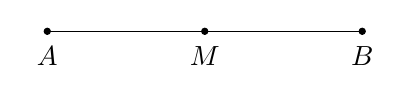
\begin{tikzpicture}[scale=1, line join=round, line cap=round, >=stealth]
				%% Khai bao diem
				\path 
				(0,0) coordinate (A)
				(2,0) coordinate (M)
				(4,0) coordinate (B)
				;
				\draw (A)--(B);
				%% vẽ điểm
				\foreach \x/\g in {A/-90,M/-90,B/-90}
				\draw[fill=black] (\x) circle (.039)+(\g:.31)
				node{$\x$};	
				
		\end{tikzpicture}}	\\
		Ta có $\overrightarrow{AB}$ và $\overrightarrow{AM}$ cùng phương.}
\end{ex}
%%=======Câu 9=======%%
\begin{ex}%[0H5V1-3]%[Dự án đề kiểm tra Toán 10 HKI NH24-25- Vũ Ngọc Ánh]%[Sở GD&ĐT Bắc Giang]
	\textit{(Trích đề HKI - Sở GD ĐT Bắc Giang - Năm học 2024 - 2025)}\\	Cho tam giác $ABC$. Có bao nhiêu vectơ khác $\overrightarrow{0}$ có điểm đầu và điểm cuối là các đỉnh của tam giác $ABC$?
	\choice
	{$3$}
	{\True $6$}
	{$9$}
	{$8$}
	\loigiai{
		Các vectơ khác vectơ $\overrightarrow{0}$ thỏa mãn là $\overrightarrow{AB}$, $\overrightarrow{AC}$, $\overrightarrow{BC}$, $\overrightarrow{BA}$, $\overrightarrow{CA}$, $\overrightarrow{CB}$.	
	}
\end{ex}
%%=======Câu 10=======%%
\begin{ex}%[Dự án đề cương 3 Khối NH24-25-Dot1-Nguyễn Tấn Tài]%[0H5H1-3]
	Cho hình chữ nhật $ABCD$ có tâm là $I$. Khẳng định nào sau đây là đúng?
	\choice
	{$\overrightarrow{IC}=\overrightarrow{DI}$}
	{\True $\overrightarrow{AI}=\overrightarrow{IC}$}
	{$\overrightarrow{BI}=\overrightarrow{DI}$}
	{$\overrightarrow{IA}=\overrightarrow{BI}$}
	\loigiai{
		\immini{Do $I$ là tâm của hình chữ nhật $ABCD$ nên $I$ là trung điểm của $AC$.\\Vậy ta có $\overrightarrow{AI}=\overrightarrow{IC}$.}
		{\begin{tikzpicture}[scale=1, line join=round, line cap=round]
				\def\d{4}
				\def\r{2.5}
				\path
				(0,0) coordinate (D) 
				(0:\d) coordinate (C)
				(90:\r) coordinate (A)
				($(A)+(C)-(D)$) coordinate (B)
				(intersection of A--C and B--D) coordinate (I)
				;
				\draw (A)--(B)--(C)--(D)--(A)--(C) (B)--(D);
				\foreach \x/\g in {A/135,B/45,C/-45,D/-135,I/-90}
				\draw[fill=black] (\x) circle (.04)+(\g:.31)
				node{$\x$};	
		\end{tikzpicture}}
	}
\end{ex}
%%=======Câu 11=======%%
\begin{ex}%[Dự án đề cương 3 Khối NH24-25-Dot1-Nguyễn Tấn Tài]%[0H5H1-3]
	Cho tứ giác $ABCD$ có $\overrightarrow{AB}=\overrightarrow{DC}$ và $\left|\overrightarrow{AB}\right|=\left|\overrightarrow{AD}\right|$ thì tứ giác $ABCD$ là hình gì?
	\choice
	{Hình thang cân}
	{\True Hình thoi}
	{Hình chữ nhật}
	{Hình vuông}
	\loigiai{
		Do $\overrightarrow{AB}=\overrightarrow{DC}$ nên $ABCD$ là hình bình hành.\\
		Mặt khác $\left|\overrightarrow{AB}\right|=\left|\overrightarrow{AD}\right|$ nên $AB=AD$.\\
		Suy ra $ABCD$ là hình thoi (\textit{hình bình hành có 2 cạnh kề bằng nhau là hình thoi}).
	}
\end{ex}
%%=======Câu 12=======%%
\begin{ex}%[Dự án đề cương 3 Khối NH24-25-Dot1-Nguyễn Tấn Tài]%[0H5N1-3]
	Cho bốn điểm phân biệt $A$, $B$, $C$, $D$ thỏa mãn $\overrightarrow{AB}=\overrightarrow{DC}$. Khẳng định nào sau đây là khẳng định \textbf{sai}?
	\choice
	{$AB=CD$}
	{$\overrightarrow{AB}$ và $\overrightarrow{DC}$ là hai vectơ cùng hướng}
	{$AC$ và $BD$ nhận cùng một điểm làm trung điểm}
	{\True $ABCD$ là hình bình hành}
	\loigiai{
		$ABCD$ là hình bình hành khi và chỉ khi bốn điểm $A$, $B$, $C$, $D$ không thẳng hàng và $\overrightarrow{AB}=\overrightarrow{DC}$.}
\end{ex}
%%=======Câu 13=======%%
\begin{ex}%[Dự án đề cương 3 Khối NH24-25-Dot1-Nguyễn Tấn Tài]%[0H5N1-2]
	Cho tam giác $ABC$ có $M$, $N$ lần lượt là trung điểm của hai cạnh $AB$ và $AC$. Khẳng định nào sau đây là khẳng định đúng?
	\choice
	{$\overrightarrow{MN}$ và $\overrightarrow{AC}$ cùng phương}
	{\True $\overrightarrow{MN}$ và $\overrightarrow{BC}$ cùng phương}
	{$\overrightarrow{MN}$ và $\overrightarrow{AB}$ cùng phương}
	{$\overrightarrow{MN}$ và $\overrightarrow{BN}$ cùng phương}
	\loigiai{
		\immini{
			Ta có $MN$ là đường trung bình của tam giác $ABC$ nên $MN\parallel BC$. Do đó hai vectơ $\overrightarrow{MN}$ và $\overrightarrow{BC}$ cùng phương.
		}
		{
			\begin{tikzpicture}[scale=1,line join=round, line cap=round,>=stealth]
				\path
				(0,0) coordinate (B) 
				(0:4) coordinate (C)
				(70:3) coordinate (A)
				($(A)!0.5!(B)$) coordinate (M)
				($(A)!0.5!(C)$) coordinate (N)
				;
				\draw (A)--(B)--(C)--(A) (M)--(N);
				\foreach \x/\g in {A/90,B/-135,C/-45,M/160,N/20}
				\draw[fill=black] (\x) circle (.04)+(\g:.31)
				node{$\x$};	
			\end{tikzpicture}
		}
	}
\end{ex}
%%=======Câu 14=======%%
\begin{ex}%[0H5N1-2]%[Dự án đề kiểm tra Toán 10 GK1-2024-2025-Nguyễn Sĩ Đạt]%[THPT Chuyên Bình Thuận - Bình Thuận]
	\textit{(Trích đề GHKI - THPT Chuyên Bình Thuận - Năm học 2024 - 2025)}\\
	Cho hình bình hành $A B C D$. Các vectơ nào dưới đây cùng phương với vectơ $\vec{A B}$?
	\choice
	{\True $\vec{B A}$, $\vec{C D}$, $\vec{D C}$}
	{$\vec{D A}$, $\vec{C D}$, $\vec{C B}$}
	{$\vec{A D}$, $\vec{C D}$, $\vec{D C}$}
	{$\vec{B A}$, $\vec{C D}$, $\vec{C B}$}
	\loigiai{
		\begin{center}
			{\begin{tikzpicture}[scale=1, font=\footnotesize, line join=round, line cap=round, >=stealth]
					\coordinate[label=below:$D$] (D) at (0,0);
					\coordinate[label=below:$C$] (C) at (3,0);
					\coordinate[label=above:$B$] (B) at (5,2);
					\coordinate[label=above:$A$] (A) at (2,2);
					\draw (A)--(B)--(C)--(D)--(A); 
			\end{tikzpicture}}
		\end{center}
		Các vectơ cùng phương với vectơ $\vec{A B}$ là $\vec{B A}$, $\vec{C D}$, $\vec{D C}$.
	}
\end{ex}
%%=======Câu 15=======%%
\begin{ex}%[0H5N1-3]%[Dự án tex hóa đề kiểm tra HKI NH24-25- Ngô Tất Thành]%[THPT - Chuyên Hùng Vương - Phú Thọ]
	\textit{(Trích đề HKI - THPT Chuyên Hùng Vương, Phú Thọ - Năm học 2024 - 2025)}\immini
	{Cho hình vuông $ABCD$ có tâm $O$ (hình vẽ).
		Vectơ $\overrightarrow{AO}$ bằng vectơ
		\choice[2]
		{$\overrightarrow{OD}$}
		{$\overrightarrow{CO}$}
		{$\overrightarrow{OB}$}
		{\True $\overrightarrow{OC}$}}
	{\begin{tikzpicture}[scale=0.8, font=\footnotesize,line join=round, line cap=round, >=stealth]
			\def\canh{3}
			\path 
			(0,0) coordinate (D)
			++(90:\canh) coordinate (A)
			++(0:\canh) coordinate (B)
			++(-90:\canh) coordinate (C)
			($(A)!1/2!(C)$) coordinate (O)
			;
			\draw (A)--(B)--(C)--(D)--(A)--(C) (B)--(D);
			\foreach \x/\y/\z in {A/B/C, D/A/B, D/C/B, C/D/A}
			{pic[draw,angle eccentricity=1.8,angle radius=2mm]{right angle = \x--\y--\z}}
			;
			\foreach \i/\g in {A/90,B/90,C/-90,D/-90,O/-90}
			\fill[black] (\i) circle(1pt)+(\g:3mm)node[scale=1]{$\i$};
	\end{tikzpicture}}
	\loigiai{
		Trong hình vuông $ABCD$, ta có
		$O$ là giao điểm của hai đường chéo $AC$ và $BD$ nên $O$ là trung điểm của $AC$.\\
		Do đó $\overrightarrow{AO} = \overrightarrow{OC}$ (vì $\vec{AO}$ và $\vec{OC}$ cùng hướng và cùng độ dài).
	}
\end{ex}

%%=======Câu 16=======%%
\begin{ex}%[Dự án đề cương 3 Khối NH24-25-Dot1-Nguyễn Tấn Tài]%[0H5H1-5]
	\immini[thm]{Cho tam giác đều $ABC$ cạnh $a$ và có trung tuyến $BM$. Độ dài của $\overrightarrow{BM}$ là
		\haicot
		{$a\sqrt{3}$}
		{$\dfrac{a\sqrt{2}}{3}$}
		{\True $\dfrac{a\sqrt{3}}{2}$}
		{$\dfrac{a\sqrt{3}}{3}$}}{
		\begin{tikzpicture}[smooth,font=\footnotesize,scale=0.8]
			\path
			(0,0) coordinate (B)
			(4,0) coordinate (C)
			($(B)!1!60:(C)$)coordinate (A)
			($(A)!0.5!(C)$)coordinate (M);
			\draw (A)--(B)--(C)--cycle (B)--(M);
			\foreach \x/\g in {A/90,B/-90,C/-90,M/0} \draw [fill=black] (\x) circle (.05) + (\g:.3) node{$\x$};
	\end{tikzpicture}}
	\loigiai{
		Trong tam giác đều $ABC$ cạnh $a$, có trung tuyến $BM=\left|\overrightarrow{BM}\right|=\dfrac{a\sqrt{3}}{2}$.}
\end{ex}
%%=======Câu 17=======%%
\begin{ex}%[Dự án đề cương 3 Khối NH24-25-Dot1-Nguyễn Tấn Tài]%[0H5N1-5] 
	\immini[thm]{Cho hình vuông $ABCD$ cạnh bằng $a$. Gọi $M$ là trung điểm của $CD$. Tính độ dài của  $\overrightarrow{AM}$.
		\haicot
		{ $\dfrac{a\sqrt{3}}{2}$}
		{\True $\dfrac{a\sqrt{5}}{2}$}
		{ $\dfrac{3a}{2}$}
		{ $\dfrac{5a}{2}$}
	}{\begin{tikzpicture}[scale=1, line join=round, line cap=round]
			\def\d{3}
			\def\r{3}
			\path
			(0,0) coordinate (D) 
			(0:\d) coordinate (C)
			(90:\r) coordinate (A)
			($(A)+(C)-(D)$) coordinate (B)
			($(D)!1/2!(C)$) coordinate (M)
			;
			\draw (A)--(B)--(C)--(D)--(A)--(M);
			\foreach \x/\g in {A/135,B/45,C/-45,D/-135,M/-90}
			\draw[fill=black] (\x) circle (.04)+(\g:.31)
			node{$\x$};	
	\end{tikzpicture}}
	\loigiai{
		Ta có $\left|\overrightarrow{AM}\right|=AM=\sqrt{AD^2+DM^2}=\sqrt{a^2+\left(\dfrac{a}{2}\right)^2}=\dfrac{a\sqrt{5}}{2} $
	}
\end{ex}
%%=======Câu 18=======%%
\begin{ex}%[0D1N1-1]%[Dự án đề kiểm tra Toán 10 GHKI NH23-24-VU Ngoc Hao]%[Lê Thánh Tông - HCM]
	\textit{(Trích đề GHKI - THPT Lê Thánh Tông - Năm học 2023 - 2024)}\\
	Cho hình thang $A B C D$ có $A B \parallel C D$. Gọi $M$ là trung điểm của đoạn $C D$. Có bao nhiêu vectơ khác vectơ-không, cùng hướng với vectơ $\overrightarrow{A B}$ và có điểm đầu, điểm cuối được lấy từ các điểm đã cho?	
	\choice
	{$5$}
	{$2$}
	{\True $3$}
	{$4$}
	\loigiai{
		\begin{center}
			\begin{tikzpicture}[scale=1, font=\footnotesize, line join=round, line cap=round, >=stealth]
				\path 
				(1,2) coordinate (A)
				(0,0) coordinate (D)
				(5,0) coordinate (C)
				(3,2) coordinate (B)
				($(D)!0.5!(C)$) coordinate (M)
				;
				\draw (D)--(A)--(B)--(C)--cycle;
				\foreach \p/\r in {A/90,D/-120,C/-60,B/60,M/-90}
				\fill (\p) circle (1.5pt) node[shift={(\r:3mm)}]{$\p$};
				
			\end{tikzpicture}
		\end{center}
		Các vectơ cùng hướng với vectơ $\overrightarrow{AB}$ là $\overrightarrow{DM}$, $\overrightarrow{MC}$, $\overrightarrow{DC}$. Vậy có $3$ vectơ cùng hướng với vectơ $\overrightarrow{AB}$.
	}
\end{ex}
%%=======Câu 19=======%%
\begin{ex}%[Dự án đề cương 3 Khối NH24-25-Dot1-Nguyễn Tấn Tài]%[0H5H1-5]
	Trong mặt phẳng cho hai điểm phân biệt $A$, $B$. Tập hợp tất cả các điểm $M$ thỏa mãn $\left|\overrightarrow{AM}\right|=\left|\overrightarrow{AB}\right|$ là hình gì?
	\choice
	{Đường trung trực của đoạn thẳng $AB$}
	{\True Đường tròn tâm $A$ bán kính $AB$}
	{Đường tròn tâm $B$ bán kính $AB$}
	{Đoạn thẳng $AB$}
	\loigiai{ 
		Ta có $\left|\overrightarrow{AM}\right|=\left|\overrightarrow{AB}\right|$ tức là khoảng cách từ $A$ đến $M$ bằng độ dài đoạn $AB$. Tập hợp các điểm $M$ thỏa mãn điều đó là đường tròn tâm $A$ bán kính $AB$.
	}
\end{ex}
%%=======Câu 20=======%%
\begin{ex}%[Dự án đề cương 3 Khối NH24-25-Dot1-Nguyễn Tấn Tài]%[0H5H1-3]
	Cho hình thang $ABCD$ có $AB$ và $CD$ song song với nhau. Phát biểu nào sau đây là đúng?
	\choice
	{$\overrightarrow{AB}=\overrightarrow{CD}$}
	{\True $\overrightarrow{AB}$ và $\overrightarrow{DC}$ cùng hướng}
	{$\overrightarrow{AB}$ và $\overrightarrow{DC}$ ngược hướng}
	{$\overrightarrow{AB}=\overrightarrow{DC}$}
	\loigiai{ 
		Vì $AB \parallel CD$ nên $\overrightarrow{AB}$ và $\overrightarrow{CD}$ cùng phương.\\
		Tuy nhiên, các vectơ này có hướng ngược nhau nên $\overrightarrow{AB}$ và $\overrightarrow{DC}$ là hai vectơ cùng hướng.
	}
\end{ex}

\Closesolutionfile{ans}

\ind{PHẦN II.} \inden{Câu trắc nghiệm đúng sai. Trong mỗi ý a), b), c), d) ở mỗi câu, học sinh chọn đúng hoặc sai.}\\
\Opensolutionfile{ans}[ans/0H5-B1-2]
\setcounter{ex}{0}
\begin{ex}%[Dự án đề cương 3 Khối NH24-25-Dot1-Nguyễn Tấn Tài]%[0H5N1-3]
	Gọi ${K}$ là trung điểm của đoạn thẳng ${PQ}$.
	\choiceTF
	{\True $\overrightarrow{QP}$ cùng phương với $\overrightarrow{QK}$}
	{$\overrightarrow{KP}=\overrightarrow{KQ}$}
	{$\left|\overrightarrow{QP}\right|=\left|\overrightarrow{QK}\right|$}
	{$\overrightarrow{QP}$ ngược hướng với $\overrightarrow{QK}$}
	\loigiai{
		\centerline{
			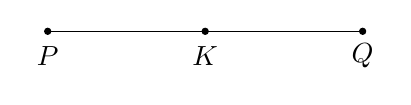
\begin{tikzpicture}[scale=1, line join=round, line cap=round, >=stealth]
				%% Khai bao diem
				\path 
				(0,0) coordinate (P)
				(2,0) coordinate (K)
				(4,0) coordinate (Q)
				;
				\draw (P)--(Q);
				%% vẽ điểm
				\foreach \x/\g in {P/-90,K/-90,Q/-90}
				\draw[fill=black] (\x) circle (.039)+(\g:.31)
				node{$\x$};	
				
		\end{tikzpicture}}
		\begin{itemchoice}
			\itemch Vì $P$, $K$, $Q$ thẳng hàng ($K$ là trung điểm của $PQ$) nên $\overrightarrow{QP}$ cùng phương với $\overrightarrow{QK}$.
			\itemch Vì $\overrightarrow{KP}$ ngược hướng với $\overrightarrow{KQ}$ nên hai vectơ không thể bằng nhau.
			\itemch $\left|\overrightarrow{QK}\right|=\dfrac{1}{2}\left|\overrightarrow{QP}\right|$, nên không bằng nhau.
			\itemch $\overrightarrow{QP}$ và $\overrightarrow{QK}$ cùng hướng.
		\end{itemchoice}
	}
\end{ex}

\begin{ex}%[Dự án đề cương 3 Khối NH24-25-Dot1-Nguyễn Tấn Tài]%[0H5N1-3]
	\immini[thm]{Cho hình bình hành ${ABCD}$ tâm $O$.
		\choiceTF
		{\True $\overrightarrow{DA}$ và $\overrightarrow{CB}$ là cùng hướng }
		{$\overrightarrow{OA}=\overrightarrow{OC}$}
		{\True $\left|\overrightarrow{OB}\right|=\left|\overrightarrow{OD}\right|$}
		{$\left|\overrightarrow{AC}\right|=\left|\overrightarrow{BD}\right|$}
	}{\begin{tikzpicture}[scale=1,line join=round,line cap=round, >=stealth]
			\def\a{4}
			\def\g{60}
			\path 
			(0,0) coordinate (A)
			(A)++(0:\a) coordinate (B)
			(B)++(\g:\a/2) coordinate (C)
			($(A)+(C)-(B)$) coordinate (D)
			(intersection of A--C and B--D) coordinate (O)
			;
			\draw 
			(A)--(B)--(C)--(D)--cycle
			(A)--(C) (B)--(D)
			;
			\foreach \x/\g in {A/135, B/-45, C/60, D/150, O/-95}{
				\draw[fill=black] (\x) circle (0.045) +(\g:0.3) node {$\x$};
			};
	\end{tikzpicture}}
	\loigiai{ 
		\begin{itemchoice}
			\itemch Vì $ABCD$ là hình bình hành nên $DA \parallel CB$ và $DA=CB$.\\
			Suy ra $\overrightarrow{DA}$ cùng hướng với $\overrightarrow{CB}$ và $\left|\overrightarrow{DA}\right|=\left|\overrightarrow{CB}\right|$.\\
			Vậy $\overrightarrow{DA}=\overrightarrow{CB}$.
			\itemch Vì $O$ là trung điểm của $AC$ nên $\overrightarrow{OA}$ và $\overrightarrow{OC}$ ngược hướng nhau.
			\itemch $O$ là trung điểm của $BD$ nên $\left|\overrightarrow{OB}\right|=\left|\overrightarrow{OD}\right|$.
			\itemch Vì $ABCD$ không là hình chữ nhật nên độ dài $AC$ và $BD$ khác nhau.
		\end{itemchoice}
	}
\end{ex}

\begin{ex}%[Dự án đề cương 3 Khối NH24-25-Dot1-Nguyễn Tấn Tài]%[0H5N1-3]
	\immini[thm]{Cho tam giác đều ${DEF}$. Gọi $M$ là trung điểm của đoạn $DE$.
		\choiceTF
		{$\overrightarrow{DE}=\overrightarrow{DF}$ }
		{$\overrightarrow{ME}=\overrightarrow{MD}$}
		{\True $\overrightarrow{ME}$ cùng phương với $\overrightarrow{ED}$}
		{ \True $\left|\overrightarrow{ED}\right|=\left|\overrightarrow{EF}\right|$ }}{
		\begin{tikzpicture}[scale=0.7, font=\footnotesize,>=stealth]
			\path
			%	Vẽ mp
			(0,0) coordinate (D)
			(3,0) coordinate (E)
			($(D)!1!60:(E)$)coordinate (F)
			($(D)!.5!(E)$)coordinate (M)
			;
			\draw (D)--(E)--(F)--(D);
			\foreach \x/\g in {D/180,E/0,F/90,M/-90}\draw[fill=black] (\x) circle (.05) +(\g:.4)node{\footnotesize$\x$};
	\end{tikzpicture}}
	\loigiai{	\begin{itemchoice}
			\itemch Vì $\overrightarrow{DE}$ không cùng phương với $\overrightarrow{DF}$ nên hai vectơ không thể bằng nhau.
			\itemch Vì $M$ là trung điểm của $DE$ nên $\overrightarrow{ME}$ và $\overrightarrow{MD}$ là hai vectơ ngược hướng (không thể bằng nhau).
			\itemch Vì $D$, $M$, $E$ thẳng hàng nên $\overrightarrow{ME}$ cùng phương với $\overrightarrow{ED}$.
			\itemch Vì $\triangle DEF$ đều nên $DE=EF$. Suy ra $\left|\overrightarrow{ED}\right|=\left|\overrightarrow{EF}\right|$.
	\end{itemchoice}}
\end{ex}

\begin{ex}%[Dự án đề cương 3 Khối NH24-25-Dot1-Nguyễn Tấn Tài]%[0H5N1-5]
	\immini[thm]{Cho hình vuông ${ABCD}$ cạnh bằng $a$, $I$ là điểm trên cạnh $BC$ thỏa $CI=\dfrac{1}{2}IB$. 
		\choiceTF
		{\True $\overrightarrow{DA}$ và $\overrightarrow{BC}$ là ngược hướng }
		{ $\overrightarrow{AC}=\overrightarrow{BD}$ }
		{$\left|\overrightarrow{AC}\right|=2a$}
		{\True $\left|\overrightarrow{AI}\right|=\dfrac{\sqrt{13}a}{3}$}}{\begin{tikzpicture}[scale=1, line join=round, line cap=round]
			\def\d{3}
			\def\r{3}
			\path
			(0,0) coordinate (D) 
			(0:\d) coordinate (C)
			(90:\r) coordinate (A)
			($(A)+(C)-(D)$) coordinate (B)
			($(C)!1/3!(B)$) coordinate (I)
			;
			\draw (A)--(B)--(C)--(D)--(A)--(I);
			\foreach \x/\g in {A/135,B/45,C/-45,D/-135,I/0}
			\draw[fill=black] (\x) circle (.04)+(\g:.31)
			node{$\x$};	
	\end{tikzpicture}}
	\loigiai{	\begin{itemchoice}
			\itemch Vì $ABCD$ là hình bình hành nên $DA \parallel BC$. Suy ra $\overrightarrow{DA}$ cùng phương với $\overrightarrow{BC}$\\
			Xét về chiều, ta có được $\overrightarrow{DA}$ ngược hướng với $\overrightarrow{BC}$.
			\itemch Hai vectơ $\overrightarrow{AC}$ và $\overrightarrow{BD}$ không cùng phương nên hai vectơ không bằng nhau.
			\itemch Độ dài đường chéo $AC$ của hình vuông là $a\sqrt{2}$. Suy ra $\left|\overrightarrow{AC}\right|=a\sqrt{2}$.
			\itemch  Đặt $CI=x$ $(x>0)$, khi đó $IB=2x$.\\
			Ta có $CI+IB=CB \Leftrightarrow 3x=a \Leftrightarrow x=\dfrac{a}{3}$.\\
			Suy ra $CI=\dfrac{a}{3}$ và $IB=\dfrac{2a}{3}$.\\
			Xét $AIB$ vuông tại $B$, áp dụng định lí Pythagore có 
			\[AB^2+BI^2=AI^2 \Rightarrow AI=\sqrt{AB^2+BI^2} =\dfrac{a\sqrt{13}}{3}.		\]
	\end{itemchoice}}
	
\end{ex}
%%=======Câu 12=======%%
\begin{ex}%[Dự án đề cương 3 Khối NH24-25-Dot1-Nguyễn Tấn Tài]%[0H5N1-5]
	Cho hình chữ nhật $ABCD$ có $O$ là giao điểm của hai đường chéo và $AB=a$, $BC=3a$.
	\choiceTF
	{\True $\left|\overrightarrow{DC}\right|=a$}
	{$\left|\overrightarrow{AD}\right|=4a$}
	{\True $\left|\overrightarrow{BD}\right|=\sqrt{10}a$}
	{\True $\left|\overrightarrow{OB}\right|=\dfrac{\sqrt{10}a}{2}$}
	\loigiai{
		\immini{\begin{itemchoice}
				\itemch Vì$ABCD$ là hình chữ nhật nên nên $CD=AB$.\\
				Suy ra $\left|\overrightarrow{DC}\right|=CD=AB=a$.
				\itemch Vì$ABCD$ là hình chữ nhật nên nên $AD=BC$.\\
				Suy ra $\left|\overrightarrow{AD}\right|=AD=BC=3a$.
				\itemch Đường chéo $BD=\sqrt{AB^2+AD^2}=\sqrt{a^2+(3a)^2}=\sqrt{10}a$.\\
				Suy ra $\left|\overrightarrow{BD}\right|=BD=a\sqrt{10}$.
				\itemch $O$ là trung điểm đường chéo $BD$ nên $OB=\dfrac{1}{2}BD=\dfrac{a\sqrt{10}}{2}$.\\
				Suy ra $\left|\overrightarrow{OB}\right|=OB=\dfrac{a\sqrt{10}}{2}$.
			\end{itemchoice}
		}{\begin{tikzpicture}[scale=1, line join=round, line cap=round]
				\def\d{4}
				\def\r{2.5}
				\path
				(0,0) coordinate (D) 
				(0:\d) coordinate (C)
				(90:\r) coordinate (A)
				($(A)+(C)-(D)$) coordinate (B)
				(intersection of A--C and B--D) coordinate (O)
				;
				\draw (A)--(B)--(C)--(D)--(A)--(C) (B)--(D);
				\foreach \x/\g in {A/135,B/45,C/-45,D/-135,O/-90}
				\draw[fill=black] (\x) circle (.04)+(\g:.31)
				node{$\x$};	
		\end{tikzpicture}}
	}
\end{ex}
\Closesolutionfile{ans}

\ind{PHẦN III.} \inden{Câu trắc nghiệm trả lời ngắn.}\\
\Opensolutionfile{ans}[ans/0H5-B1-3]
\setcounter{ex}{0}
\begin{ex}%[Dự án đề cương 3 Khối NH24-25-Dot1-Nguyễn Tấn Tài]%[0H5H1-2]
	Cho các vectơ như hình vẽ. Có bao nhiêu cặp vectơ cùng phương xuất hiện trong hình?\\
	\shortans[oly]{$8$}
	\begin{center}
		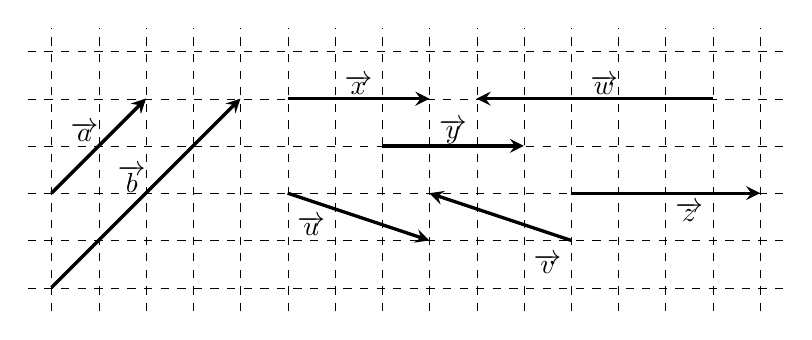
\begin{tikzpicture}[line width=1.2,>=stealth,scale=0.6]
			\draw[step=1,ultra thin,dashed](-0.5,-0.5)grid(15.5,5.5);
			\draw[->](0,2)--(2,4);
			\draw[->](0,0)--(4,4);
			\draw[->](5,4)--(8,4);
			\draw[->](5,2)--(8,1);
			\draw[->](7,3)--(10,3);
			\draw[->](0,2)--(2,4);
			\draw[->](14,4)--(9,4);
			\draw[->](11,2)--(15,2);
			\draw[->](11,1)--(8,2);
			\node at (0.7,3.3) {$\overrightarrow{a}$};
			\node at (1.7,2.3) {$\overrightarrow{b}$};
			\node at (5.5,1.3) {$\overrightarrow{u}$};
			\node at (10.5,0.5) {$\overrightarrow{v}$};
			\node at (13.5,1.6) {$\overrightarrow{z}$};
			\node at (6.5,4.3) {$\overrightarrow{x}$};
			\node at (8.5,3.3) {$\overrightarrow{y}$};
			\node at (11.7,4.3) {$\overrightarrow{w}$};
		\end{tikzpicture}
	\end{center}
	\loigiai{
		Có $8$ cặp vectơ cùng phương xuất hiện trong hình gồm: $\overrightarrow{a}$ và $\overrightarrow{b}$, $\overrightarrow{x}$ và $\overrightarrow{y}$, $\overrightarrow{x}$ và $\overrightarrow{z}$, $\overrightarrow{x}$ và $\overrightarrow{w}$, $\overrightarrow{y}$ và $\overrightarrow{z}$, $\overrightarrow{y}$ và $\overrightarrow{w}$, $\overrightarrow{z}$ và $\overrightarrow{w}$, $\overrightarrow{u}$ và $\overrightarrow{v}$.}
\end{ex}

\begin{ex}%[Dự án đề cương 3 Khối NH24-25-Dot1-Nguyễn Tấn Tài]%[0H5N1-5]
	Cho hình vuông $ABCD$ có độ dài cạnh bằng $3$ cm. Tính độ dài của $\overrightarrow{AC}$. (kết quả làm tròn đến hai chữ số thập phân)\\
	\shortans[oly]{$4{,}24$}
	\loigiai{
		\immini{
			$\left|\overrightarrow{AC}\right|=AC=\sqrt{AB^2+BC^2}=\sqrt{3^2+3^2}=3\sqrt{2} \approx 4{,}24$ cm.
		}{
			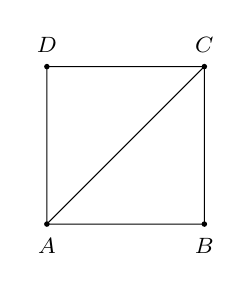
\begin{tikzpicture}[scale=1, font=\footnotesize, line join=round, line cap=round,>=stealth]
				\draw (0,0) rectangle (2,2) (0,0)--(2,2);
				\foreach\i/\j/\goc/\diem in{0/0/-90/A,2/0/-90/B,2/2/90/C,0/2/90/D}
				\fill(\i,\j) circle(1.0pt) node[shift={(\goc:8pt)}]{$\diem$};
			\end{tikzpicture}
		}
	}
\end{ex}

\begin{ex}%[Dự án đề cương 3 Khối NH24-25-Dot1-Nguyễn Tấn Tài]%[0H5N1-5]
	\immini{
		Cho hình chữ nhật $ABCD$ có cạnh $AB=3$, $BC=4$. Độ dài của $\overrightarrow{DB}$ bằng bao nhiêu?\\
		\shortans[oly]{$5$}
	}{
		\begin{tikzpicture}[scale=0.8, font=\footnotesize, line join=round, line cap=round, >=stealth]
			\path	(0,0) coordinate (A)++(0:3) coordinate (D)
			($(A)+(-90:2)$) coordinate (B)
			($(B)+(D)-(A)$) coordinate (C)
			;
			\draw (A)--(B)--(C)--(D)--(A);
			\foreach \x/\g in {A/130,D/60,C/-30,B/-150}  \fill (\x) circle (1pt)+(\g:.3)node[scale=0.8]{$\x$};	
		\end{tikzpicture}
	}
	\loigiai{
		Áp dụng định lí Pythagore cho tam giác vuông $ABC$ ta có 
		\[ AC=\sqrt{AB^2+BC^2}=\sqrt{3^2+4^2}=5. \]
		Vì $ABCD$ là hình chữ nhật nên $\left|\overrightarrow{DB}\right|=\left|\overrightarrow{AC}\right|=AC=5$.
	}
\end{ex}

\begin{ex}%[Dự án đề cương 3 Khối NH24-25-Dot1-Nguyễn Tấn Tài]%[0H5N1-5]
	Cho tam giác $ABC$ đều cạnh bằng $1$, trọng tâm $G$. Độ dài của $\overrightarrow{AG}$ bằng bao nhiêu? (kết quả làm tròn đến hai chữ số thập phân)\\
	\shortans[oly]{$0{,}58$}
	\loigiai{
		\immini
		{
			Gọi $I$ là trung điểm của $BC \Rightarrow AI=\dfrac{\sqrt{3}}{2}$.\\
			Ta có $AG=\dfrac{2}{3}AI=\dfrac{2}{3} \cdot \dfrac{\sqrt{3}}{2}=\dfrac{\sqrt{3}}{3} \Rightarrow \left|\overrightarrow{AG}\right|=\dfrac{\sqrt{3}}{3}\approx 0,58$.
		}
		{
			\begin{tikzpicture}[>=stealth,line cap=round,line join=round,scale=.6,font=\footnotesize]
				\tkzDefPoints{-2/-3/B,4/-3/C}
				\tkzDefPointBy[rotation=center B angle 60](C)    \tkzGetPoint{A}
				\coordinate (I) at ($(C)!0.5!(B)$);
				\tkzCentroid(A,B,C)    \tkzGetPoint{G}
				\tkzDrawPolygon(A,B,C)
				\tkzDrawPoints[fill=black](A,B,C,I,G)
				\tkzDrawSegments(G,I)
				\draw[blue,->](A)--(G);
				\tkzLabelPoints[left](G,B)
				\tkzLabelPoints[above](A)
				\tkzLabelPoints[below](I)
				\tkzLabelPoints[right](C)
			\end{tikzpicture}
		}
	}
\end{ex}

\begin{ex}%[Dự án đề cương 3 Khối NH24-25-Dot1-Nguyễn Tấn Tài]%[0H5N1-5]
	Cho tam giác $ABC$ đều có cạnh bằng $8$. Gọi $G$ là trọng tâm tam giác $ABC$ và $I$ là trung điểm của $AG$. Độ dài của $\overrightarrow{AI}$ (làm tròn kết quả đến hàng phần trăm) bằng bao nhiêu?\\
	\shortans[oly]{$2{,}31$}
	\loigiai{
		\immini{
			Gọi $M$ là trung điểm của $BC$. Ta có
			\[\begin{array}{l} {\left|\overrightarrow{AG}\right|=AG=\dfrac{2}{3} AM=\dfrac{2}{3} \sqrt{AB^2-BM^2}=\dfrac{2}{3} \sqrt{8^2-\dfrac{8^2}{4}}=\dfrac{8\sqrt{3}}{3}} \\ {\left|\overrightarrow{AI}\right|=AI=\dfrac{AG}{2}=\dfrac{4\sqrt{3}}{3} \approx 2{,}31} \end{array}
			\]
		}{
			\begin{tikzpicture}[scale=1, font=\footnotesize, line join=round, line cap=round, >=stealth]
				\path	(0,0) coordinate (B)++(0:3) coordinate (C)
				($(B)+(60:3)$) coordinate (A)
				($(B)!1/2!(C)$) coordinate (M)
				($(A)!2/3!(M)$) coordinate (G)
				($(A)!1/2!(G)$) coordinate (I)
				;
				\draw (A)--(B)--(C)--(A)--(M);
				\foreach \x/\g in {A/90,B/-150,C/-30,I/0,G/0,M/-90}  \fill (\x) circle (1pt)+(\g:.3)node[scale=1]{$\x$};	
			\end{tikzpicture}
		}
	}
\end{ex}

\Closesolutionfile{ans}
\ind{PHẦN IV.} \inden{Bài tập tự luận.}\\
\Opensolutionfile{ans}[ans/0H5-B1-3]
\setcounter{ex}{0}
\begin{ex}%[Dự án đề cương 3 Khối NH24-25-Dot1-Nguyễn Tấn Tài]%[0H5H1-6] 
	Tìm các lực cùng hướng và ngược hướng trong số các lực đẩy được biểu diễn bằng các vectơ trong hình dưới đây.
	\begin{center}
		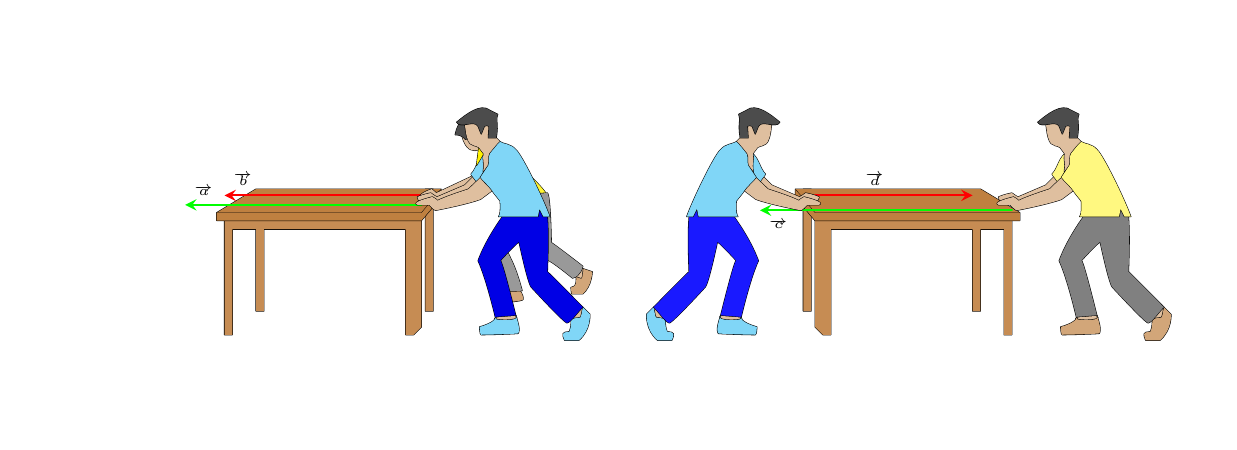
\begin{tikzpicture}[line join=round, line cap=round,>=stealth,font=\footnotesize,scale=1]
			\begin{scope}[shift={(0,0)}, scale=1, rotate=0]
				\clip (-4.5,-2.5) rectangle (4.5,2.5);
				\begin{pgfinterruptboundingbox}
					%------------Bàn
					\def\O{  
						%---chân bàn
						(.4,.05)--(.5,.05)--(.5,-1.3)--(.4,-1.4)--cycle
						(.65,.45)--(.65,-1.1)--(.55,-1.1)--(.55,.45)--cycle
						(-2,.05)--(-2,-1.4)--(-1.9,-1.4)--(-1.9,-.06)--(-1.6,-.06)--(-1.6,-1.1)--(-1.5,-1.1)--(-1.5,-.06)--(.3,-.06)--(.3,-1.4)--(.4,-1.4)--(.4,-.06)--(.4,.05)--cycle
						;}
					\draw \O;
					\fill[brown!90] \O;
					%--mặt bàn
					\def\Z{  
						(.5,.15)--(.75,.45)--(-1.6,.45)--(-2.1,.15)--cycle
						(.5,.15)--(.5,.05)--(-2.1,.05)--(-2.1,.15)--cycle
						(.5,.15)--(.5,.05)--(.75,.35)--(.75,.45)--cycle
						;}
					\draw \Z;
					\fill[brown] \Z;
					\draw[ultra thin] (-2.1,.15)--(.5,.15)--(.75,.45);
					%---------------vectơ
					\draw[->,color=green,thick] (.5,.25)--(-2.5,.25);
					\draw[->,color=red,thick] (.5,.37)--(-2,.37);
					\node at (-2.5,.25) [above right]{\tiny $\overrightarrow{a}$};
					\node at (-2,.37) [above right]{\tiny $\overrightarrow{b}$};
					%------------Mặt người sau
					\def\E{ 
						(1,1.2)
						..controls +(-80:0.24) and +(175:0.06) .. (1.18,.94)
						..controls +(5:0.1) and +(-120:0) .. (1.28,1.04)
						%..controls +(80:0.2) and +(-140:0) .. (1.1,1.4)
						;}
					\draw \E;
					\fill[brown!50!] \E;
					%------------Tóc người sau
					\def\D{ 
						(1.1,1.1)
						..controls +(-170:0) and +(20:0) .. (1.06,1.08)
						..controls +(160:0) and +(0:0.1) .. (.93,1.14)
						..controls +(80:0.2) and +(-140:0) .. (1.1,1.4)
						;}
					\draw \D;
					\fill[black!70!] \D;
					%------------Áo người sau
					\def\F{  (1.8,.37)
						..controls +(180:0) and +(-10:0) .. (2.1,.37)
						..controls +(120:0.1) and +(-35:0) .. (1.9,.6)--cycle
						;}
					\draw \F;
					\fill[yellow!80] \F;
					%------------Bàn chân (1) người sau
					\def\J{  (1.78,-.96)
						..controls +(15:0.05) and +(-160:0) ..  (1.73,-0.8)
						..controls +(180:0.05) and +(-10:0) .. (1.6,-0.8)
						..controls +(-160:0.05) and +(30:0) .. (1.45,-.96)
						..controls +(180:0.05) and +(-165:0.2) .. (1.78,-.96)
						;}
					\draw \J;
					\fill[brown!70!] \J;
					%------------Bàn chân (2) người sau
					\def\G{  (2.46,-.66)
						..controls +(-120:0) and +(70:0.1) .. (2.45,-.78)
						..controls +(180:0) and +(5:0) .. (2.4,-.8)
						..controls +(-170:0) and +(125:0.01) .. (2.41,-.88)
						..controls +(0:0.06) and +(18:0) .. (2.55,-.88)
						..controls +(40:0.15) and +(-165:0) .. (2.67,-.6)
						..controls +(140:0) and +(-35:0) .. (2.55,-.56)
						..controls +(140:0) and +(-35:0.01) .. (2.53,-.68)
						..controls +(175:0) and +(15:0.01) .. (2.46,-.66)
						;}
					\draw \G;
					\fill[brown!70!] \G;
					
					\def\K{  (2.55,-.56)
						..controls +(140:0) and +(-35:0.01) .. (2.53,-.68)
						..controls +(175:0) and +(15:0.01) .. (2.46,-.66)
						;}
					\draw \K;
					\fill[brown!50] \K;
					%------------Quần người sau
					\def\F{  (1.4,-.84)
						..controls +(-10:0.1) and +(-10:0) .. (1.78,-.84)
						..controls +(105:0.4) and +(-70:0.15) .. (1.55,-.25)--cycle
						;}
					\draw \F;
					\fill[gray!80] \F;
					\def\G{  (2.1,-.45)
						..controls +(-10:0.05) and +(-10:0) .. (2.42,-.68)
						..controls +(10:0.1) and +(170:0) .. (2.55,-.53)
						..controls +(170:0) and +(-30:0.05) .. (2.15,-.23)
						..controls +(160:0) and +(-35:0.05) .. (2.1,.4)
						..controls +(160:0) and +(-35:0) .. (1.8,.38)--cycle
						;}
					\draw \G;
					\fill[gray!80] \G;
					%------------Da chân sau người trước
					\def\S{  (2.55,-1.05)
						..controls +(140:0) and +(-35:0.01) .. (2.52,-1.18)
						..controls +(175:0) and +(15:0.01) .. (2.4,-1.2)
						;}
					\draw \S;
					\fill[brown!50!] \S;
					
					%------------Bàn chân (2) người trước
					\def\T{  (2.4,-1.2)
						..controls +(-120:0) and +(70:0.1) .. (2.38,-1.36)
						..controls +(180:0) and +(5:0) .. (2.32,-1.37)
						..controls +(-170:0.05) and +(25:0) .. (2.32,-1.47)
						..controls +(0:0.05) and +(18:0) .. (2.5,-1.47)
						..controls +(40:0.2) and +(-165:0) .. (2.64,-1.14)
						..controls +(140:0) and +(-35:0) .. (2.55,-1.05)
						..controls +(140:0) and +(-35:0.01) .. (2.52,-1.18)
						..controls +(175:0) and +(15:0.01) .. (2.4,-1.2)
						;}
					\draw \T;
					\fill[cyan!50!] \T;
					
					%------------Tay người sau
					\def\Q{  (1.2,.64)
						..controls +(-160:0) and +(40:0) ..  (.69,.4)
						..controls +(150:0) and +(-40:0) ..  (.63,.45)
						..controls +(-160:0.3) and +(50:0) ..  (.55,.3)
						..controls +(-160:0.1) and +(50:0) ..   (1.2,.4)
						--cycle
						;}
					\draw \Q;
					\fill[brown!50!] \Q;
					%------------Tay phải người trước
					\def\V{  (1.15,.6)
						..controls +(-160:0) and +(40:0) ..  (1.05,.5)
						..controls +(-160:0) and +(40:0) ..  (.7,.35)
						..controls +(170:0.02) and +(-25:0) ..  (.62,.4)
						..controls +(-170:0.1) and +(40:0) ..  (.45,.35)
						..controls +(-80:0.05) and +(-140:0) ..  (.48,.3)
						..controls +(0:0.2) and +(180:0) ..  (1.18,.3)
						..controls +(0:0.1) and +(180:0) ..  (1.2,.64)
						--cycle
						;}
					\draw \V;
					\fill[brown!50!] \V;
					
					%------------Áo phải người trước
					\def\B{ (1.25,.6)
						..controls +(-150:0) and +(30:0) .. (1.21,.53)
						..controls +(110:0.01) and +(-70:0.01) .. (1.13,.64)
						..controls +(45:0.1) and +(-135:0.12) .. (1.29,.9)
						..controls +(-100:0.1) and +(80:0.12) .. (1.285,.675)--cycle
						;}
					\draw \B;
					\fill[cyan!50!] \B;
					
					\def\M{ 
						(1.29,.9)..controls +(160:0.02) and +(-20:0.01) ..(1.23,.98)--(1.2,.75)--cycle;}
					\draw \M;
					\fill[yellow]\M;
					
					%------------Cổ trước
					\def\C{ 
						(1.29,.9)
						..controls +(-100:0.1) and +(80:0.12) ..(1.285,.675)
						..controls +(35:0) and +(-145:0) .. (1.35,.75)
						..controls +(70:.05) and +(-120:.05) .. (1.37,.9)
						..controls +(50:.05) and +(-140:.05) .. (1.5,1.05)
						..controls +(140:0) and +(-40:0) .. (1.45,1.1)
						..controls +(180:0) and +(0:0) .. (1.35,1.1)
						..controls +(80:0) and +(-110:0) .. (1.36,1.25)
						..controls +(165:0.04) and +(15:0.04) .. (1.3,1.25)
						..controls +(-120:0) and +(60:0) .. (1.26,1.15)
						..controls +(130:0) and +(-50:0) .. (1.22,1.25)
						..controls +(120:0.1) and +(-60:.1) .. (0.95,1.3)
						..controls +(-35:0) and +(145:0) .. (1,1.27)
						..controls +(120:0.1) and +(-60:.1) .. (1.05,1.3)
						..controls +(-85:0.35) and +(150:.1) .. (1.23,.98)
						%..controls +(-100:0) and +(80:0) .. (1.2,.75)
						--cycle
						;}
					\draw \C;
					\fill[brown!50] \C;
					
					%------------Tóc người trước
					\def\D{ 
						(1.45,1.1)
						..controls +(180:0) and +(0:0) .. (1.35,1.1)
						..controls +(80:0) and +(-110:0) .. (1.36,1.25)
						..controls +(165:0.04) and +(15:0.04) .. (1.3,1.25)
						..controls +(-120:0) and +(60:0) .. (1.26,1.15)
						..controls +(130:0) and +(-50:0) .. (1.22,1.25)
						..controls +(120:0.1) and +(-60:.1) .. (0.95,1.3)
						..controls +(40:.15) and +(140:.15) .. (1.37,1.45)
						..controls +(80:0) and +(-110:0) .. (1.47,1.4)
						..controls +(-110:0.1) and +(80:.2) .. (1.45,1.1)
						;}
					\draw \D;
					\fill[black!70!] \D;
					%------------Quần người trước
					\def\F{  (1.53,.1)
						..controls +(-120:0) and +(70:0.3) .. (1.22,-.46)
						..controls +(-65:0.25) and +(120:0) .. (1.44,-1.18)
						..controls +(0:.05) and +(-15:.05) .. (1.7,-1.16)
						..controls +(-130:0) and +(70:0.05) .. (1.5,-.46)
						..controls +(40:0) and +(-150:0.05) .. (1.74,-.22)
						..controls +(-80:0) and +(150:0.05) .. (1.9,-.8)
						..controls +(-40:0) and +(165:0.05) .. (2.35,-1.25)
						..controls +(10:0.05) and +(-145:0.05) .. (2.55,-1.05)
						..controls +(165:0) and +(-40:0.05) .. (2.1,-.6)
						..controls +(85:0) and +(-70:0.15) .. (2.08,.21)--cycle
						;}
					\draw \F;
					\fill[blue!90!black] \F;
					%------------Tay (1) người trước
					\def\J{  (1.42,.45)
						..controls +(15:0.01) and +(-160:0) ..  (1.25,.32)
						..controls +(-160:0.2) and +(20:0) ..  (.68,.18)
						..controls +(170:0.02) and +(-25:0) ..  (.6,.25)
						..controls +(180:0.1) and +(0:0) ..  (.45,.25)
						..controls +(160:0.1) and +(-140:0) ..  (.64,.35)
						..controls +(-30:0.1) and +(150:0) ..  (.7,.3)
						..controls +(30:0.1) and +(-150:0) ..  (1.1,.45)
						..controls +(50:0.02) and +(150:0) ..  (1.3,.64)
						;}
					\draw \J;
					\fill[brown!50!] \J;
					%------------Áo người trước
					\def\A{  (1.42,.4)
						..controls +(120:.1) and +(-60:.05) .. (1.25,.6)
						..controls +(40:0) and +(-140:0) .. (1.35,.75)
						..controls +(70:.05) and +(-120:.05) .. (1.37,.9)
						..controls +(50:.05) and +(-140:.05) .. (1.5,1.05)
						..controls +(-35:.05) and +(130:.1) .. (1.7,.95)
						..controls +(-40:.1) and +(110:.25) .. (2.13,.1)
						..controls +(180:0) and +(0:0) .. (2.05,.1)
						..controls +(140:0) and +(-40:0) .. (2,.2)
						..controls +(-110:0) and +(70:0) .. (1.98,.1)
						..controls +(180:0) and +(0:0) .. (1.48,.1)
						..controls +(45:0.05) and +(-135:0) .. (1.5,.3)--cycle
						;}
					\draw \A;
					\fill[cyan!50!] \A;
					
					%------------Bàn chân người trước
					\def\R{ 
						(1.7,-1.16)
						..controls +(-40:.12) and +(-160:0.12) .. (1.45,-1.18)--cycle
						;}
					\draw \R;
					\fill[brown!50!] \R;
					
					\def\T{  (1.45,-1.18)
						..controls +(-160:0) and +(15:0.2) .. (1.24,-1.3)
						..controls +(-80:0) and +(170:0.02) .. (1.26,-1.4)
						..controls +(0:0.05) and +(-10:0.05) .. (1.73,-1.38)
						..controls +(100:0) and +(-70:0.2) .. (1.7,-1.16)
						..controls +(-40:.12) and +(-160:0.12) .. (1.45,-1.18)
						;}
					\draw \T;
					\fill[cyan!50!] \T;
					
				\end{pgfinterruptboundingbox}
			\end{scope}
			\begin{scope}[shift={(6,0)}, scale=1, rotate=0]
				\clip (-4.5,-2.5) rectangle (4.5,2.5);
				\begin{pgfinterruptboundingbox}
					
					%------------Bàn
					\def\O{  
						%---chân bàn
						(.4,.05)--(.5,.05)--(.5,-1.3)--(.4,-1.4)--cycle
						(.65,.45)--(.65,-1.1)--(.55,-1.1)--(.55,.45)--cycle
						(-2,.05)--(-2,-1.4)--(-1.9,-1.4)--(-1.9,-.06)--(-1.6,-.06)--(-1.6,-1.1)--(-1.5,-1.1)--(-1.5,-.06)--(.3,-.06)--(.3,-1.4)--(.4,-1.4)--(.4,-.06)--(.4,.05)--cycle
						;}
					\draw[rotate=180,yscale=-1] \O;
					\fill[brown!90,rotate=180,yscale=-1] \O;
					%--mặt bàn
					\def\Z{  
						(.5,.15)--(.75,.45)--(-1.6,.45)--(-2.1,.15)--cycle
						(.5,.15)--(.5,.05)--(-2.1,.05)--(-2.1,.15)--cycle
						(.5,.15)--(.5,.05)--(.75,.35)--(.75,.45)--cycle
						
						;}
					\draw[rotate=180,yscale=-1] \Z;
					\fill[brown,rotate=180,yscale=-1] \Z;
					\draw[ultra thin,rotate=180,yscale=-1] (-2.1,.15)--(.5,.15)--(.75,.45);
					%---------------vectơ
					\draw[->,color=green,rotate=180,yscale=-1,thick] (-2,.18)--(1.2,.18);
					\draw[->,color=red,rotate=180,yscale=-1,thick] (.5,.37)--(-1.5,.37);
					\node at (-1.2,.18)[below right]{\tiny $\overrightarrow{c}$};
					\node at (.5,.37) [above left]{\tiny $\overrightarrow{d}$};
					
					%------------Da chân sau người trước
					\def\S{  (2.55,-1.05)
						..controls +(140:0) and +(-35:0.01) .. (2.52,-1.18)
						..controls +(175:0) and +(15:0.01) .. (2.4,-1.2)
						;}
					\draw[rotate=180,yscale=-1] \S;
					\fill[brown!50!,rotate=180,yscale=-1] \S;
					
					%------------Bàn chân (2) người trước
					\def\T{  (2.4,-1.2)
						..controls +(-120:0) and +(70:0.1) .. (2.38,-1.36)
						..controls +(180:0) and +(5:0) .. (2.32,-1.37)
						..controls +(-170:0.05) and +(25:0) .. (2.32,-1.47)
						..controls +(0:0.05) and +(18:0) .. (2.5,-1.47)
						..controls +(40:0.2) and +(-165:0) .. (2.64,-1.14)
						..controls +(140:0) and +(-35:0) .. (2.55,-1.05)
						..controls +(140:0) and +(-35:0.01) .. (2.52,-1.18)
						..controls +(175:0) and +(15:0.01) .. (2.4,-1.2)
						;}
					\draw[rotate=180,yscale=-1] \T;
					\fill[cyan!50!,rotate=180,yscale=-1] \T;
					
					%------------Tay phải người trước
					\def\V{  (1.15,.6)
						..controls +(-160:0) and +(40:0) ..  (1.05,.5)
						..controls +(-160:0) and +(40:0) ..  (.7,.35)
						..controls +(170:0.02) and +(-25:0) ..  (.62,.4)
						..controls +(-170:0.1) and +(40:0) ..  (.45,.35)
						..controls +(-80:0.05) and +(-140:0) ..  (.48,.3)
						..controls +(0:0.2) and +(180:0) ..  (1.18,.3)
						..controls +(0:0.1) and +(180:0) ..  (1.2,.64)
						--cycle
						;}
					\draw[rotate=180,yscale=-1] \V;
					\fill[brown!50!,rotate=180,yscale=-1] \V;
					
					%------------Áo phải người trước
					\def\B{ (1.25,.6)
						..controls +(-150:0) and +(30:0) .. (1.21,.53)
						..controls +(110:0.01) and +(-70:0.01) .. (1.13,.64)
						..controls +(45:0.1) and +(-135:0.12) .. (1.29,.9)
						..controls +(-100:0.1) and +(80:0.12) .. (1.285,.675)--cycle
						;}
					\draw[rotate=180,yscale=-1] \B;
					\fill[cyan!50!,rotate=180,yscale=-1] \B;
					
					%------------Cổ trước
					\def\C{ 
						(1.29,.9)
						..controls +(-100:0.1) and +(80:0.12) ..(1.285,.675)
						..controls +(35:0) and +(-145:0) .. (1.35,.75)
						..controls +(70:.05) and +(-120:.05) .. (1.37,.9)
						..controls +(50:.05) and +(-140:.05) .. (1.5,1.05)
						..controls +(140:0) and +(-40:0) .. (1.45,1.1)
						..controls +(180:0) and +(0:0) .. (1.35,1.1)
						..controls +(80:0) and +(-110:0) .. (1.36,1.25)
						..controls +(165:0.04) and +(15:0.04) .. (1.3,1.25)
						..controls +(-120:0) and +(60:0) .. (1.26,1.15)
						..controls +(130:0) and +(-50:0) .. (1.22,1.25)
						..controls +(120:0.1) and +(-60:.1) .. (0.95,1.3)
						..controls +(-35:0) and +(145:0) .. (1,1.27)
						..controls +(120:0.1) and +(-60:.1) .. (1.05,1.3)
						..controls +(-85:0.35) and +(150:.1) .. (1.23,.98)
						%..controls +(-100:0) and +(80:0) .. (1.2,.75)
						--cycle
						;}
					\draw[rotate=180,yscale=-1] \C;
					\fill[brown!50,rotate=180,yscale=-1] \C;
					
					%------------Tóc người trước
					\def\D{ 
						(1.45,1.1)
						..controls +(180:0) and +(0:0) .. (1.35,1.1)
						..controls +(80:0) and +(-110:0) .. (1.36,1.25)
						..controls +(165:0.04) and +(15:0.04) .. (1.3,1.25)
						..controls +(-120:0) and +(60:0) .. (1.26,1.15)
						..controls +(130:0) and +(-50:0) .. (1.22,1.25)
						..controls +(120:0.1) and +(-60:.1) .. (0.95,1.3)
						..controls +(40:.15) and +(140:.15) .. (1.37,1.45)
						..controls +(80:0) and +(-110:0) .. (1.47,1.4)
						..controls +(-110:0.1) and +(80:.2) .. (1.45,1.1)
						;}
					\draw[rotate=180,yscale=-1] \D;
					\fill[black!70!,rotate=180,yscale=-1] \D;
					%------------Quần người trước
					\def\F{  (1.53,.1)
						..controls +(-120:0) and +(70:0.3) .. (1.22,-.46)
						..controls +(-65:0.25) and +(120:0) .. (1.44,-1.18)
						..controls +(0:.05) and +(-15:.05) .. (1.7,-1.16)
						..controls +(-130:0) and +(70:0.05) .. (1.5,-.46)
						..controls +(40:0) and +(-150:0.05) .. (1.74,-.22)
						..controls +(-80:0) and +(150:0.05) .. (1.9,-.8)
						..controls +(-40:0) and +(165:0.05) .. (2.35,-1.25)
						..controls +(10:0.05) and +(-145:0.05) .. (2.55,-1.05)
						..controls +(165:0) and +(-40:0.05) .. (2.1,-.6)
						..controls +(85:0) and +(-70:0.15) .. (2.08,.21)--cycle
						;}
					\draw[rotate=180,yscale=-1] \F;
					\fill[blue!90!,rotate=180,yscale=-1] \F;
					%------------Tay (1) người trước
					\def\J{  (1.42,.45)
						..controls +(15:0.01) and +(-160:0) ..  (1.25,.32)
						..controls +(-160:0.2) and +(20:0) ..  (.68,.18)
						..controls +(170:0.02) and +(-25:0) ..  (.6,.25)
						..controls +(180:0.1) and +(0:0) ..  (.45,.25)
						..controls +(160:0.1) and +(-140:0) ..  (.64,.35)
						..controls +(-30:0.1) and +(150:0) ..  (.7,.3)
						..controls +(30:0.1) and +(-150:0) ..  (1.1,.45)
						..controls +(50:0.02) and +(150:0) ..  (1.3,.64)
						;}
					\draw[rotate=180,yscale=-1] \J;
					\fill[brown!50!,rotate=180,yscale=-1] \J;
					%------------Áo người bên trái
					\def\A{  (1.42,.4)
						..controls +(120:.1) and +(-60:.05) .. (1.25,.6)
						..controls +(40:0) and +(-140:0) .. (1.35,.75)
						..controls +(70:.05) and +(-120:.05) .. (1.37,.9)
						..controls +(50:.05) and +(-140:.05) .. (1.5,1.05)
						..controls +(-35:.05) and +(130:.1) .. (1.7,.95)
						..controls +(-40:.1) and +(110:.25) .. (2.13,.1)
						..controls +(180:0) and +(0:0) .. (2.05,.1)
						..controls +(140:0) and +(-40:0) .. (2,.2)
						..controls +(-110:0) and +(70:0) .. (1.98,.1)
						..controls +(180:0) and +(0:0) .. (1.48,.1)
						..controls +(45:0.05) and +(-135:0) .. (1.5,.3)--cycle
						;}
					\draw[rotate=180,yscale=-1] \A;
					\fill[cyan!50!,rotate=180,yscale=-1] \A;
					
					%------------Bàn chân người trước
					\def\R{ 
						(1.7,-1.16)
						..controls +(-40:.12) and +(-160:0.12) .. (1.45,-1.18)--cycle
						;}
					\draw[rotate=180,yscale=-1] \R;
					\fill[brown!50!,rotate=180,yscale=-1] \R;
					
					\def\T{  (1.45,-1.18)
						..controls +(-160:0) and +(15:0.2) .. (1.24,-1.3)
						..controls +(-80:0) and +(170:0.02) .. (1.26,-1.4)
						..controls +(0:0.05) and +(-10:0.05) .. (1.73,-1.38)
						..controls +(100:0) and +(-70:0.2) .. (1.7,-1.16)
						..controls +(-40:.12) and +(-160:0.12) .. (1.45,-1.18)
						;}
					\draw[rotate=180,yscale=-1] \T;
					\fill[cyan!50!,rotate=180,yscale=-1] \T;
					
					%%%%%%%%%%%%%%%%%%%%%%%Người bên phải 
					%------------Da chân sau người trước
					\def\S{  (2.55,-1.05)
						..controls +(140:0) and +(-35:0.01) .. (2.52,-1.18)
						..controls +(175:0) and +(15:0.01) .. (2.4,-1.2)
						;}
					\draw[xshift=1.38cm] \S;
					\fill[brown!50!,xshift=1.38cm] \S;
					
					%------------Bàn chân (2) người trước
					\def\T{  (2.4,-1.2)
						..controls +(-120:0) and +(70:0.1) .. (2.38,-1.36)
						..controls +(180:0) and +(5:0) .. (2.32,-1.37)
						..controls +(-170:0.05) and +(25:0) .. (2.32,-1.47)
						..controls +(0:0.05) and +(18:0) .. (2.5,-1.47)
						..controls +(40:0.2) and +(-165:0) .. (2.64,-1.14)
						..controls +(140:0) and +(-35:0) .. (2.55,-1.05)
						..controls +(140:0) and +(-35:0.01) .. (2.52,-1.18)
						..controls +(175:0) and +(15:0.01) .. (2.4,-1.2)
						;}
					\draw[xshift=1.38cm] \T;
					\fill[brown!70!,xshift=1.38cm] \T;
					
					%------------Tay phải người trước
					\def\V{  (1.15,.6)
						..controls +(-160:0) and +(40:0) ..  (1.05,.5)
						..controls +(-160:0) and +(40:0) ..  (.7,.35)
						..controls +(170:0.02) and +(-25:0) ..  (.62,.4)
						..controls +(-170:0.1) and +(40:0) ..  (.45,.35)
						..controls +(-80:0.05) and +(-140:0) ..  (.48,.3)
						..controls +(0:0.2) and +(180:0) ..  (1.18,.3)
						..controls +(0:0.1) and +(180:0) ..  (1.2,.64)
						--cycle
						;}
					\draw[xshift=1.38cm] \V;
					\fill[brown!50!,xshift=1.38cm] \V;
					
					%------------Áo phải người trước
					\def\B{ (1.25,.6)
						..controls +(-150:0) and +(30:0) .. (1.21,.53)
						..controls +(110:0.01) and +(-70:0.01) .. (1.13,.64)
						..controls +(45:0.1) and +(-135:0.12) .. (1.29,.9)
						..controls +(-100:0.1) and +(80:0.12) .. (1.285,.675)--cycle
						;}
					\draw[xshift=1.38cm] \B;
					\fill[yellow!50!,xshift=1.38cm] \B;
					
					%------------Cổ trước
					\def\C{ 
						(1.29,.9)
						..controls +(-100:0.1) and +(80:0.12) ..(1.285,.675)
						..controls +(35:0) and +(-145:0) .. (1.35,.75)
						..controls +(70:.05) and +(-120:.05) .. (1.37,.9)
						..controls +(50:.05) and +(-140:.05) .. (1.5,1.05)
						..controls +(140:0) and +(-40:0) .. (1.45,1.1)
						..controls +(180:0) and +(0:0) .. (1.35,1.1)
						..controls +(80:0) and +(-110:0) .. (1.36,1.25)
						..controls +(165:0.04) and +(15:0.04) .. (1.3,1.25)
						..controls +(-120:0) and +(60:0) .. (1.26,1.15)
						..controls +(130:0) and +(-50:0) .. (1.22,1.25)
						..controls +(120:0.1) and +(-60:.1) .. (0.95,1.3)
						..controls +(-35:0) and +(145:0) .. (1,1.27)
						..controls +(120:0.1) and +(-60:.1) .. (1.05,1.3)
						..controls +(-85:0.35) and +(150:.1) .. (1.23,.98)
						%..controls +(-100:0) and +(80:0) .. (1.2,.75)
						--cycle
						;}
					\draw[xshift=1.38cm] \C;
					\fill[brown!50,xshift=1.38cm] \C;
					
					%------------Tóc người trước
					\def\D{ 
						(1.45,1.1)
						..controls +(180:0) and +(0:0) .. (1.35,1.1)
						..controls +(80:0) and +(-110:0) .. (1.36,1.25)
						..controls +(165:0.04) and +(15:0.04) .. (1.3,1.25)
						..controls +(-120:0) and +(60:0) .. (1.26,1.15)
						..controls +(130:0) and +(-50:0) .. (1.22,1.25)
						..controls +(120:0.1) and +(-60:.1) .. (0.95,1.3)
						..controls +(40:.15) and +(140:.15) .. (1.37,1.45)
						..controls +(80:0) and +(-110:0) .. (1.47,1.4)
						..controls +(-110:0.1) and +(80:.2) .. (1.45,1.1)
						;}
					\draw[xshift=1.38cm] \D;
					\fill[black!70!,xshift=1.38cm] \D;
					%------------Quần người trước
					\def\F{  (1.53,.1)
						..controls +(-120:0) and +(70:0.3) .. (1.22,-.46)
						..controls +(-65:0.25) and +(120:0) .. (1.44,-1.18)
						..controls +(0:.05) and +(-15:.05) .. (1.7,-1.16)
						..controls +(-130:0) and +(70:0.05) .. (1.5,-.46)
						..controls +(40:0) and +(-150:0.05) .. (1.74,-.22)
						..controls +(-80:0) and +(150:0.05) .. (1.9,-.8)
						..controls +(-40:0) and +(165:0.05) .. (2.35,-1.25)
						..controls +(10:0.05) and +(-145:0.05) .. (2.55,-1.05)
						..controls +(165:0) and +(-40:0.05) .. (2.1,-.6)
						..controls +(85:0) and +(-70:0.15) .. (2.08,.21)--cycle
						;}
					\draw[xshift=1.38cm] \F;
					\fill[black!50!,xshift=1.38cm] \F;
					%------------Tay (1) người trước
					\def\J{  (1.42,.45)
						..controls +(15:0.01) and +(-160:0) ..  (1.25,.32)
						..controls +(-160:0.2) and +(20:0) ..  (.68,.18)
						..controls +(170:0.02) and +(-25:0) ..  (.6,.25)
						..controls +(180:0.1) and +(0:0) ..  (.45,.25)
						..controls +(160:0.1) and +(-140:0) ..  (.64,.35)
						..controls +(-30:0.1) and +(150:0) ..  (.7,.3)
						..controls +(30:0.1) and +(-150:0) ..  (1.1,.45)
						..controls +(50:0.02) and +(150:0) ..  (1.3,.64)
						;}
					\draw[xshift=1.38cm] \J;
					\fill[brown!50!,xshift=1.38cm] \J;
					%------------Áo người trước
					\def\A{  (1.42,.4)
						..controls +(120:.1) and +(-60:.05) .. (1.25,.6)
						..controls +(40:0) and +(-140:0) .. (1.35,.75)
						..controls +(70:.05) and +(-120:.05) .. (1.37,.9)
						..controls +(50:.05) and +(-140:.05) .. (1.5,1.05)
						..controls +(-35:.05) and +(130:.1) .. (1.7,.95)
						..controls +(-40:.1) and +(110:.25) .. (2.13,.1)
						..controls +(180:0) and +(0:0) .. (2.05,.1)
						..controls +(140:0) and +(-40:0) .. (2,.2)
						..controls +(-110:0) and +(70:0) .. (1.98,.1)
						..controls +(180:0) and +(0:0) .. (1.48,.1)
						..controls +(45:0.05) and +(-135:0) .. (1.5,.3)--cycle
						;}
					\draw[xshift=1.38cm] \A;
					\fill[yellow!50!,xshift=1.38cm] \A;
					
					%------------Bàn chân người trước
					\def\R{ 
						(1.7,-1.16)
						..controls +(-40:.12) and +(-160:0.12) .. (1.45,-1.18)--cycle
						;}
					\draw[xshift=1.38cm] \R;
					\fill[brown!50!,xshift=1.38cm] \R;
					
					\def\T{  (1.45,-1.18)
						..controls +(-160:0) and +(15:0.2) .. (1.24,-1.3)
						..controls +(-80:0) and +(170:0.02) .. (1.26,-1.4)
						..controls +(0:0.05) and +(-10:0.05) .. (1.73,-1.38)
						..controls +(100:0) and +(-70:0.2) .. (1.7,-1.16)
						..controls +(-40:.12) and +(-160:0.12) .. (1.45,-1.18)
						;}
					\draw[xshift=1.38cm] \T;
					\fill[brown!70!,xshift=1.38cm] \T;
					
				\end{pgfinterruptboundingbox}
			\end{scope}
		\end{tikzpicture}
	\end{center}
	\loigiai{
		Ta có
		\begin{enumerate}
			\item $\overrightarrow{a}$ và $\overrightarrow{b}$ cùng hướng.
			\item $\overrightarrow{c}$ và $\overrightarrow{d}$ ngược hướng.
		\end{enumerate}
	}
\end{ex}

\begin{ex}%[Dự án đề cương 3 Khối NH24-25-Dot1-Nguyễn Tấn Tài]%[0H5V1-6] 
	Tìm các lực ngược hướng trong số các lực tác động vào máy bay trong hình bên dưới.
	\begin{center}
		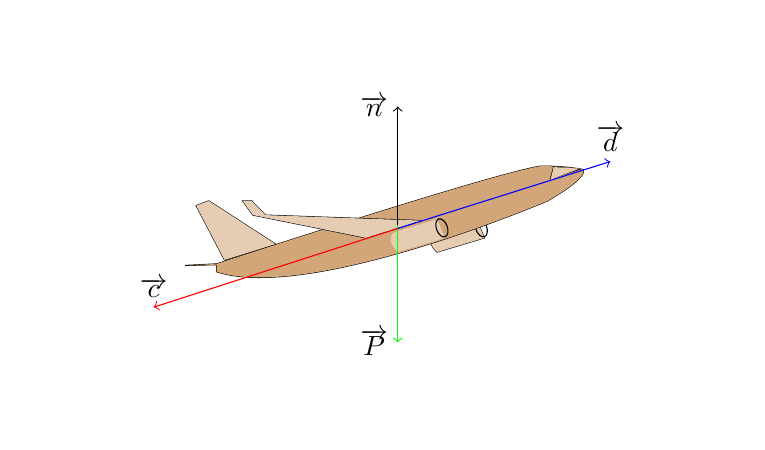
\begin{tikzpicture}
			\clip (-4.5,-2.5) rectangle (4.5,2.5);
			\begin{pgfinterruptboundingbox}
				
				%Đuôi máy bay
				\def\D{  (-2,-.45)--(-2.36,.24)--(-2.2,.3)--(-1.35,-.25)--cycle
					;}
				\draw \D;
				\fill[brown!40!] \D;
				
				%Quạt máy bay
				\def\Q{  (.15,-.1)
					..controls +(-140:0.1) and +(140:0.1) .. (.2,-.35)--(.8,-.17)--(.7,.07)--cycle
					
					;}
				\draw \Q;
				\draw[xshift=.5cm] \Q;
				\fill[brown!40!,xshift=.5cm] \Q;
				%---------elip2
				\draw[rotate=-70,xshift=-.23cm,yshift=1.27cm] (.7,-.1) ellipse (.12cm and .07cm);
				
				%Thân máy bay
				\def\T{  (-2.1,-.5)
					..controls +(40:0) and +(-170:0.7) .. (2,.74)
					..controls +(-40:0) and +(170:0.3) .. (2.55,.7)
					..controls +(-150:0) and +(30:.65) .. (2.1,.3)
					..controls +(-150:0) and +(-18:1.25) .. (-2.1,-.6)
					..controls +(90:0) and +(-90:0) .. (-2.1,-.51)
					-- (-2.5,-.52)--cycle;
				}
				\draw \T;
				\fill[brown!70!] \T;
				%Cánh máy bay
				\def\C{  (.5,.05)
					..controls +(170:0) and +(-10:0) .. (-1.48,.12)
					..controls +(-80:0) and +(170:0.02) .. (-1.65,.3)
					..controls +(180:0) and +(0:0) .. (-1.77,.3)
					..controls +(-80:0) and +(110:0) .. (-1.64,.12)
					..controls +(-35:0) and +(145:0) .. (-.2,-.17)
					--cycle
					;}
				\draw \C;
				\fill[brown!40!] \C;
				%Quạt sau
				\fill[brown!40!] \Q;
				%---------------vectơ
				\draw[->,color=green] (.2,0)--(.2,-1.5);
				\draw[->,color=black] (.2,0)--(.2,1.5);
				\draw[->,color=blue] (.2,-.05)--(2.9,0.8);
				\draw[->,color=red] (.2,-.05)--(-2.9,-1.05);
				\node at (.2,-1.5)[left]{$\overrightarrow{P}$};
				\node at (.2,1.5)[left]{$\overrightarrow{n}$};
				\node at (-2.9,-1.05)[above]{$\overrightarrow{c}$};
				\node at (2.9,0.8)[above]{$\overrightarrow{d}$};
				%----elip 1
				\draw[rotate=-70,xshift=-.4cm,yshift=.8cm] (.7,-.1) ellipse (.12cm and .07cm);
				%Ô cửa
				\draw (2.18,0.73)--(2.5,0.7)--(2.14,0.58)--cycle;
				\fill[brown!40!](2.18,0.73)--(2.51,0.71)--(2.14,0.57)--cycle;
				
			\end{pgfinterruptboundingbox}
		\end{tikzpicture}
	\end{center}
	\loigiai{
		Quan sát hình vẽ, ta thấy lực nâng $ \overrightarrow{n}$ ngược hướng với trọng lực $\overrightarrow{P}$; lực cản $\overrightarrow{c}$ ngược hướng với lực đẩy $ \overrightarrow{d}$.
	}
\end{ex}
\begin{ex}%[Dự án đề cương 3 Khối NH24-25-Dot1-Nguyễn Tấn Tài]%[0H5H1-2]
	\immini{
		Quan sát hình bên và gọi tên các vectơ:
		\begin{enumerate}[a)]
			\item Cùng phương với vectơ $\overrightarrow{x}$.
			\item Cùng hướng với vectơ $\overrightarrow{a}$.
			\item Ngược hướng với vectơ $\overrightarrow{u}$.
		\end{enumerate}
	}{
		\begin{tikzpicture}[scale=.8, font=\footnotesize, line join=round, line cap=round,>={Stealth[length=2mm]}]
			\def\xmin{0} \def\xmax{13}
			\def\ymin{0} \def\ymax{7} 
			\draw[color=gray!50,dashed] (\xmin,\ymin) grid (\xmax,\ymax); 
			\draw[->] (1,6)--(2,4);
			\draw (1.5,5) node [left] {$\overrightarrow{a}$};
			\draw[->] (3,6)--(4.5,3);
			\draw (3,4) node [above right] {$\overrightarrow{b}$};
			\draw[->] (6,6)--(11,6);
			\draw(8.5,6) node [above] {$\overrightarrow{z}$};
			\draw[->] (6,3)--(8,5);
			\draw(7,4) node [left] {$\overrightarrow{u}$};
			\draw[->] (10,5)--(8,3);
			\draw(9,4) node [left] {$\overrightarrow{v}$};
			\draw[->] (8,2)--(10,2);
			\draw(9,2) node [above] {$\overrightarrow{y}$};
			\draw[->] (2,1)--(5,1);
			\draw(3.5,1) node [above] {$\overrightarrow{x}$};
			\draw[->] (12,1)--(6,1);
			\draw(9,1) node [above] {$\overrightarrow{w}$};
			%	\draw (6.5,-.5) node{Hình 8};
			\fill (1,6) circle (2pt) (3,6)circle (2pt) (6,6)circle (2pt) (6,3)circle (2pt) (10,5)circle (2pt) (2,1)circle (2pt) (12,1)circle (2pt);
		\end{tikzpicture}
	}
	\loigiai{
		\begin{enumerate}[a)]
			\item Cùng phương với vectơ $\overrightarrow{x}$ là $\overrightarrow{y}$, $\overrightarrow{z}$, $\overrightarrow{w}$.
			\item Cùng hướng với vectơ $\overrightarrow{a}$ là $\overrightarrow{b}$.
			\item Ngược hướng với vectơ $\overrightarrow{u}$ là $\overrightarrow{v}$.
		\end{enumerate}	
	}
\end{ex}
\begin{ex}%[Dự án đề cương 3 Khối NH24-25-Dot1-Nguyễn Tấn Tài]%[0H5H1-2]
	Hãy chỉ ra các cặp vectơ cùng hướng, ngược hướng, bằng nhau trong hình dưới đây.
	\begin{center}
		\begin{tikzpicture}[scale=.8, font=\footnotesize, line join=round, line cap=round,>={Stealth[length=2mm]}]
			\def\xmin{0} \def\xmax{10}
			\def\ymin{0} \def\ymax{6} 
			\draw[color=gray!50,dashed] (\xmin,\ymin) grid (\xmax,\ymax); 
			\draw[->] (2,5)--(1,3);
			\draw (1,5) node [below right] {$\overrightarrow{a}$};
			\draw[->] (3,5)--(1,1);
			\draw (3,3) node [above left] {$\overrightarrow{b}$};
			\draw[->] (5,5)--(8,5);
			\draw(6,5) node [above right] {$\overrightarrow{y}$};
			\draw[->] (6,4)--(8,3);
			\draw(7,4) node [below right] {$\overrightarrow{v}$};
			\draw[->] (9,2)--(5,2);
			\draw(8,2) node [above left] {$\overrightarrow{x}$};
			\draw[->] (3,2)--(5,1);
			\draw(4,2) node [below right] {$\overrightarrow{u}$};
			%	\draw (6.5,-.5) node{Hình 17};
			\fill (2,5) circle (2pt) (3,5)circle (2pt) (5,5)circle (2pt) (6,4)circle (2pt) (9,2)circle (2pt) (3,2)circle (2pt);
		\end{tikzpicture}
	\end{center}
	\loigiai{
		Ta có 
		\begin{itemize}
			\item Các cặp vectơ cùng hướng là $\overrightarrow{a}$ và $ \overrightarrow{b}$, $\overrightarrow{u}$ và $\overrightarrow{v}$.
			\item Cặp vectơ ngược hướng là $\overrightarrow{x}$ và $\overrightarrow{y}$
			\item Cặp vectơ bằng nhau là $\overrightarrow{u}$ và $\overrightarrow{v}$.
		\end{itemize}
	}
\end{ex}

%\begin{ex}%[Dự án đề cương 3 Khối NH24-25-Dot1-Nguyễn Tấn Tài]%[0H1Y1-1]
%	\begin{enumerate}
	%		\item Bạn hãy tìm sự khác biệt giữa hai đại lượng sau:
	%		\begin{itemize}
		%			\item Bác Ba có số tiền là $20$ triệu đồng.
		%			\item Một cơn bão di chuyển với vận tốc $20$ km/h theo hướng đông bắc.
		%		\end{itemize}
	%		\item Trong các đại lượng sau, đại lượng nào cần được biểu diễn bởi vectơ?\\
	%		Giá tiền, lực, thể tích, tuổi, độ dịch chuyển, vận tốc.
	%	\end{enumerate}
%	\loigiai{
	%		\begin{enumerate}
		%			\item Sự khác biệt giữa hai đại lượng:
		%			\begin{itemize}
			%				\item Bác Ba có số tiền là $20$ triệu đồng là đại lượng chỉ có độ lớn, không có hướng.
			%				\item Một cơn bão di chuyển với vận tốc $ 20$ km/h theo hướng đông bắc là đại lượng có cả độ lớn và hướng.
			%			\end{itemize} 
		%			\item Đại lượng \lq\lq lực\rq\rq\,, \lq\lq độ dịch chuyển\rq\rq\ được biểu diễn bởi vectơ.
		%		\end{enumerate}
	%	}
%\end{ex}

\begin{ex}%[Dự án đề cương 3 Khối NH24-25-Dot1-Nguyễn Tấn Tài]%[0H5H1-2]
	\immini{
		Cho hình thang $ ABCD$ có hai cạnh đáy là $ AB$ và $ DC$ (hình bên). Điểm $ M$ nằm trên đoạn $ DC$.
		\begin{enumerate}
			\item Gọi tên các vectơ cùng hướng với vectơ $ \overrightarrow{AB}$.
			\item Gọi tên các vectơ ngược hướng với vectơ $ \overrightarrow{DM}$.
	\end{enumerate}}
	{
		\begin{tikzpicture}[scale=.7, font=\footnotesize, line join=round, line cap=round,>={Stealth[length=2mm]}]
			\draw (0,0) node [below left] {$ D$}--(6,0) node [below right] {$ C$}--(4,3) node [above] {$ B$}--(1,3) node [above] {$ A$}--cycle (1.5,0) node [below] {$ M$};
			\fill (0,0) circle (2pt) (6,0) circle (2pt) (4,3) circle (2pt) (1,3) circle (2pt) (1.5,0) circle (2pt);
			%	\draw (2.5,-.5) node{Hình 15};
		\end{tikzpicture}
	}
	\loigiai{
		\begin{enumerate}
			\item Các vectơ cùng hướng với vectơ $ \overrightarrow{AB}$ là $ \overrightarrow{DM}$, $ \overrightarrow{MC}$, $ \overrightarrow{DC}$.
			\item Các vectơ ngược hướng với vectơ $ \overrightarrow{DM}$ là $ \overrightarrow{MD}$, $ \overrightarrow{CM}$, $ \overrightarrow{CD}$, $ \overrightarrow{BA}$.
		\end{enumerate}
	}
\end{ex}
\begin{ex}%[Dự án đề cương 3 Khối NH24-25-Dot1-Nguyễn Tấn Tài]%[0H5H1-1] 
	\immini{
		Cho hình vuông $ ABCD$ có tâm $ O$ và có cạnh bằng $ a$ (hình bên). 
		\begin{enumerate}
			\item Tìm trong hình hai vectơ bằng nhau và có độ dài bằng $ \dfrac{a\sqrt{2}}{2}$.
			\item Tìm trong hình hai vectơ đối nhau và có độ dài bằng $ a\sqrt{2}$.
	\end{enumerate}}
	{
		\begin{tikzpicture}[scale=0.7, font=\footnotesize, line join=round, line cap=round, >=stealth]
			\def\dc{4} % cạnh BC
			\def\da{4} % cạnh BA
			\def\h{4} % đường cao
			\def\gocD{90} % góc B của đáy
			\coordinate[label=below:$D$] (D) at (0,0);
			\coordinate[label=above:$A$] (A) at (\gocD:\da);
			\coordinate[label=below:$C$] (C) at (\dc,0);
			\coordinate[label=above:$B$] (B) at ($(A)+(C)-(D)$);
			\draw (A)--(D)--(C)--(B)--cycle (A)--(C) (B)--(D);
			\foreach \diem in {A,B,C,D}	\fill (\diem)circle(1.5pt);
			\coordinate[label=below:$O$] (O) at ($(A)!.5!(C)$);
			\coordinate[label=left:$a$] (I) at ($(A)!.5!(D)$);
		\end{tikzpicture}
	}
	\loigiai{
		\begin{enumerate}
			\item Ta có 
			\begin{itemize}
				\item $ \overrightarrow{AO}=\overrightarrow{OC}$ và $ \left|\overrightarrow{AO}\right|=\left|\overrightarrow{OC} \right|=\dfrac{a\sqrt{2}}{2}$,
				\item $ \overrightarrow{OA}=\overrightarrow{CO}$ và $ \left|\overrightarrow{OA}\right|=\left|\overrightarrow{CO} \right|=\dfrac{a\sqrt{2}}{2}$,
				\item $ \overrightarrow{BO}=\overrightarrow{OD}$ và $ \left|\overrightarrow{BO}\right|=\left|\overrightarrow{OD} \right|=\dfrac{a\sqrt{2}}{2}$,
				\item $ \overrightarrow{OB}=\overrightarrow{DO}$ và $ \left|\overrightarrow{OB}\right|=\left|\overrightarrow{DO} \right|=\dfrac{a\sqrt{2}}{2}$.
			\end{itemize}
			\item Ta có 
			\begin{itemize}
				\item $ \overrightarrow{AC}=-\overrightarrow{CA}$ và $ \left|\overrightarrow{AC}\right|=\left|\overrightarrow{CA} \right|=a\sqrt{2}$,
				\item$ \overrightarrow{BD}=-\overrightarrow{DB}$ và $ \left|\overrightarrow{BD}\right|=\left|\overrightarrow{DB} \right|=a\sqrt{2}$.
			\end{itemize}
		\end{enumerate}
	}
\end{ex}
\begin{ex}%[Dự án đề cương 3 Khối NH24-25-Dot1-Nguyễn Tấn Tài]%[0H5H1-3] 
	Cho tứ giác $ ABCD$. Chứng minh rằng tứ giác đó là hình bình hành khi và chỉ khi $ \overrightarrow{AB}=\overrightarrow{DC}$.
	\loigiai{
		Ta có $ ABCD$ là hình bình hành $\Leftrightarrow \heva{&AB\parallel DC\\&AB=DC\\&\overrightarrow{AB} \text{ cùng hướng với }\overrightarrow{DC}} \Leftrightarrow \overrightarrow{AB}=\overrightarrow{DC}$.
	}
\end{ex}
\begin{ex}%[Dự án đề cương 3 Khối NH24-25-Dot1-Nguyễn Tấn Tài]%[0H5H1-5]
	\immini{Cho hình vuông $ABCD$ có cạnh bằng $\dfrac{\sqrt{2}}{2}$, hai đường chéo cắt nhau tại $O$. Tìm độ dài của các vectơ $\overrightarrow{CA}$, $\overrightarrow{BD}$, $\overrightarrow{OA}$, $\overrightarrow{AO}$.}
	{
		\begin{tikzpicture}[scale=0.7, font=\footnotesize, line join=round, line cap=round, >=stealth]
			\def\dc{4} % cạnh BC
			\def\da{4} % cạnh BA
			\def\h{4} % đường cao
			\def\gocD{90} % góc B của đáy
			\coordinate[label=below:$D$] (D) at (0,0);
			\coordinate[label=above:$A$] (A) at (\gocD:\da);
			\coordinate[label=below:$C$] (C) at (\dc,0);
			\coordinate[label=above:$B$] (B) at ($(A)+(C)-(D)$);
			\draw (A)--(D)--(C)--(B)--cycle (A)--(C) (B)--(D);
			\foreach \diem in {A,B,C,D}	\fill (\diem)circle(1.5pt);
			\coordinate[label=right:$O$] (O) at ($(A)!.5!(C)$);
			\coordinate[label=left:$\dfrac{\sqrt{2}}{2}$] (I) at ($(A)!.5!(D)$);
		\end{tikzpicture}
	}
	\loigiai{
		Ta có: $CA=1$, $BD=1$, $AO=\dfrac{1}{2}$.\\
		Suy ra $\left|\overrightarrow{CA} \right|=1$, $\left|\overrightarrow{BD} \right|=1$, $\left|\overrightarrow{OA} \right|= \left|\overrightarrow{AO} \right|=\dfrac{1}{2}$.
	}
\end{ex}

\begin{ex}%[Dự án đề cương 3 Khối NH24-25-Dot1-Nguyễn Tấn Tài]%[0H5H1-3] 
	Cho tam giác $ABC$ vuông tại $A$, $AB=3a$, $AC=4a$. Tính độ dài của $\overrightarrow{BC}$.
	\loigiai{
		Ta có $\left| \overrightarrow{BC}\right|= BC=\sqrt{AB^2+AC^2}=\sqrt{(3a)^2+(4a)^2}=5a$.
	}
\end{ex}

\begin{ex}
	Cho tứ giác $ABCD$. Gọi $M$, $N$, $P$, $Q$ lần lượt là trung diểm $AB$, $BC$, $CD$, $D A$. Chứng minh rằng $\overrightarrow{M N}=\overrightarrow{Q P}$.	
	\loigiai{
		\immini{Vì $MN$ là đường trung bình của $\triangle ABC$ nên $MN \parallel AC$ và $MN=\dfrac{AC}{2}$.\\
			Vì $QP$ là đường trung bình của $\triangle ADC$ nên $QP \parallel AC$ và $QP=\dfrac{AC}{2}$.\\	
			Do đó $MN=QP$ và $MN \parallel QP$.\\
			Vậy $\overrightarrow{MN}=\overrightarrow{QP}$.
		}
		{\begin{tikzpicture}[scale=0.7, font=\footnotesize, line join=round, line cap=round, >=stealth]
				\path 
				(0,0) coordinate (D)
				(5,0) coordinate (C)
				(4.6,3) coordinate (B)
				(1.3,2.6) coordinate (A)
				($(A)!1/2!(B)$) coordinate (M)
				($(B)!1/2!(C)$) coordinate (N)
				($(C)!1/2!(D)$) coordinate (P)
				($(D)!1/2!(A)$) coordinate (Q)
				;
				\draw (A)--(B)--(C)--(D)--(A)--(C) (M)--(N) (P)--(Q);
				\foreach \x/\g in {A/135,B/45,C/-45,D/-135,M/90,N/0,Q/180,P/-95}
				\draw[fill=black] (\x) circle (.036)+(\g:.3)
				node{$\x$};	
		\end{tikzpicture}}
	}
\end{ex}

\Closesolutionfile{ans}


